%&pdflatex
\documentclass[final,leqno]{siamltex}
%\documentclass[10pt,onecolumn]{article}
\usepackage[top=2cm,bottom=3cm,left=3.5cm,right=3.5cm]{geometry}
\usepackage[utf8]{inputenc}
\usepackage{amsmath,amssymb,amsfonts,mathrsfs}
%\let\proof\relax 
%\let\endproof\relax
\usepackage{listings}
\usepackage{array}
\usepackage{mathtools}
\usepackage{dsfont}
\usepackage{graphicx}
\usepackage{pdfpages}
\usepackage[textsize=footnotesize,color=green]{todonotes}
\usepackage{algorithm, algorithmic}
\usepackage{array}
\usepackage{bm}
\usepackage{tikz}
\usepackage{subfigure}
\usepackage[normalem]{ulem}

%\usepackage{lineno}
%\pagewiselinenumbers
%\usepackage{uselinenofix}


\newcommand{\bs}[1]{\boldsymbol{#1}}

\newcommand{\equaldef}{\stackrel{\mathrm{def}}{=}}

\newcommand{\tablab}[1]{\label{tab:#1}}
\newcommand{\tabref}[1]{Table~\ref{tab:#1}}

\newcommand{\theolab}[1]{\label{theo:#1}}
\newcommand{\theoref}[1]{\ref{theo:#1}}
\newcommand{\eqnlab}[1]{\label{eq:#1}}
\newcommand{\eqnref}[1]{\eqref{eq:#1}}
\newcommand{\seclab}[1]{\label{sec:#1}}
\newcommand{\secref}[1]{\ref{sec:#1}}
\newcommand{\lemlab}[1]{\label{lem:#1}}
\newcommand{\lemref}[1]{\ref{lem:#1}}

\newcommand{\mb}[1]{\mathbf{#1}}
\newcommand{\mbb}[1]{\mathbb{#1}}
\newcommand{\mc}[1]{\mathcal{#1}}
\newcommand{\nor}[1]{\left\| #1 \right\|}
\newcommand{\snor}[1]{\left| #1 \right|}
\newcommand{\LRp}[1]{\left( #1 \right)}
\newcommand{\LRs}[1]{\left[ #1 \right]}
\newcommand{\LRa}[1]{\left\langle #1 \right\rangle}
\newcommand{\LRc}[1]{\left\{ #1 \right\}}
\newcommand{\LRb}[1]{\left| #1 \right|}

\newcommand{\tanbui}[2]{\textcolor{blue}{\sout{#1}} \textcolor{red}{#2}}
\newcommand{\Grad} {\ensuremath{\nabla}}
\newcommand{\Div} {\ensuremath{\nabla\cdot}}
\newcommand{\Nel} {\ensuremath{{N^\text{el}}}}
\newcommand{\jump}[1] {\ensuremath{\LRs{\!\left[#1\right]\!}}}
\newcommand{\uh}{\widehat{u}}
\newcommand{\fnh}{\widehat{f}_n}
\renewcommand{\L}{L^2\LRp{\Omega}}
\newcommand{\pO}{\partial\Omega}
\newcommand{\Gh}{\Gamma_h}
\newcommand{\Gm}{\Gamma_{-}}
\newcommand{\Gp}{\Gamma_{+}}
\newcommand{\Go}{\Gamma_0}
\newcommand{\Oh}{\Omega_h}

\newcommand{\eval}[2][\right]{\relax
  \ifx#1\right\relax \left.\fi#2#1\rvert}

\def\etal{{\it et al.~}}

\newcommand{\vect}[1]{\ensuremath\boldsymbol{#1}}
\newcommand{\tensor}[1]{\underline{\vect{#1}}}
\newcommand{\del}{\Delta}
\let\grad\relax
\newcommand{\grad}{\nabla}
\newcommand{\curl}{\grad \times}
\renewcommand{\div}{\grad \cdot}
\newcommand{\ip}[1]{\left\langle #1 \right\rangle}
\newcommand{\eip}[1]{a\left( #1 \right)}
\newcommand{\pd}[2]{\frac{\partial#1}{\partial#2}}
\newcommand{\pdd}[2]{\frac{\partial^2#1}{\partial#2^2}}

\newcommand{\circone}{\ding{192}}
\newcommand{\circtwo}{\ding{193}}
\newcommand{\circthree}{\ding{194}}
\newcommand{\circfour}{\ding{195}}
\newcommand{\circfive}{\ding{196}}

\def\arr#1#2#3#4{\left[
\begin{array}{cc}
#1 & #2\\
#3 & #4\\
\end{array}
\right]}
\def\vecttwo#1#2{\left[
\begin{array}{c}
#1\\
#2\\
\end{array}
\right]}
\def\vectthree#1#2#3{\left[
\begin{array}{c}
#1\\
#2\\
#3\\
\end{array}
\right]}
\def\vectfour#1#2#3#4{\left[
\begin{array}{c}
#1\\
#2\\
#3\\
#4\\
\end{array}
\right]}

%\newtheorem{proposition}{Proposition}
%\newtheorem{corollary}{Corollary}
%\newtheorem{theorem}{Theorem}
%\newtheorem{lemma}{Lemma}

\newcommand{\G} {\Gamma}
\newcommand{\Gin} {\Gamma_{in}}
\newcommand{\Gout} {\Gamma_{out}}

\newtheorem{remark}{Remark}

%\title{A minimum-residual finite element method for the convection-diffusion equation}
\title{A Dual Petrov-Galerkin finite element method for the convection-diffusion equation}
\author{Jesse Chan, John A. Evans, Weifeng Qiu}
\date{}
\begin{document}

\maketitle

\begin{abstract}
We present a minimum-residual finite element method for convection-diffusion problems in a higher order, adaptive, continuous Galerkin setting.  The method borrows concepts from both the Discontinuous Petrov-Galerkin (DPG) method by Demkowicz and Gopalakrishnan \cite{DPG2} and the method of variational stabilization by Cohen, Dahmen, and Welper \cite{DahmenVariationalStabilization}, and it can also be interpreted as a variational multiscale method in which the fine-scales are defined through a dual-orthogonality condition.  A key ingredient in the method is the proper choice of norm used to measure the residual, and we present two choices which are observed to be robust in both convection and diffusion-dominated regimes, as well as a proof of stability for quasi-uniform meshes and a method for the weak imposition of boundary conditions.  Numerically obtained convergence rates in 2D are reported, and benchmark numerical examples are given to illustrate the behavior of the method.  
\end{abstract}

%\begin{keywords}\end{keywords}
%\begin{AMS}\end{AMS}

\section{Introduction}

It is well known that the standard Galerkin finite element method performs very poorly for the convection-diffusion equation -- in the convection-dominated case, it experiences spurious oscillations in the solution that grow as $\epsilon \rightarrow 0$.  The problem is connected back to a loss of discrete coercivity with respect to the standard $H^1$ norm \cite{roos2008robust}.  The concept of \textit{stabilized} methods was introduced in order to combat such oscillations, the most popular of which is the Streamline Upwind Petrov-Galerkin (SUPG) method \cite{SUPG}.  The method can be interpreted as adding a sufficient amount of artificial viscosity in the streamline direction in order to restore discrete coercivity with respect to a new ``streamline-diffusion'' norm \cite{johnsonCrosswind}.  SUPG is also an example of a residual-based stabilization, where the stabilization mechanism disappears as the strong residual of the equation is satisfied.  

A connection can be drawn between residual-based stabilized methods and Petrov-Galerkin schemes, where the trial (approximating) functions and test (weighting) functions are allowed to differ.  Specifically, the SUPG method can be interpreted as a modification of standard test functions\footnote{We note that one cannot recover the SUPG formulation beginning with the strong form of the equations and the SUPG test functions; the interpretation of SUPG as a Petrov-Galerkin scheme holds only locally, on element interiors.}, biasing them in the upwind direction based on mesh size, order of polynomial approximation, the magnitude of convection, and the diffusion parameter.  More recently, the concept of Petrov-Galerkin methods has been connected to a novel \textit{minimum residual} framework -- it is shown that the minimization of a specific residual corresponding to a variational formulation naturally leads to the concept of optimal test functions \cite{overviewDPG}.  Additionally, this framework has been exploited as an alternative method of proving stability for more standard methods in the least squares finite element community \cite{lsqUltraWeak}.

Optimal test functions resulting from residual minimization were first implemented by Demkowicz and Gopalakrishnan in \cite{DPG2,DPG1}.  The connection between stabilization and least squares/minimum residual methods has been observed previously \cite{GLS}; however, the Discontinuous Petrov-Galerkin method distinguishes itself by measuring the residual of the operator form of the equation, which is posed in the dual space.  Independently, Cohen, Dahmen and Welper introduced an alternative saddle-point formulation of such a minimum residual method in \cite{DahmenVariationalStabilization}, which alluded to a Variational Multiscale (VMS) perspective \cite{VMS1,VMS2,HughesVMS}.  We refer to the method of Cohen, Dahmen, and Welper as a Dual Petrov-Galerkin method, which distinguishes itself from the Discontinuous Petrov-Galerkin method in that it does not use a broken test space.  

The goal of this paper is three-fold.  The first is to present a method which borrows concepts from each of these recent works and to derive a more detailed connection between the Petrov-Galerkin, stabilized, and VMS perspectives of minimum-residual methods.  The second is to demonstrate that the proposed method is robust in both convection and diffusion-dominated regimes provided the dual norm used to measure the residual is chosen intelligently.  The last goal is to show that the method is stable for arbitrary higher order and adaptive meshes and easily implemented using existing finite element codes and technologies. %and extendable to three-dimensional convection-diffusion problems.

\section{A minimum-residual method}

Our starting point is the minimization of some measure of error over a finite-dimensional space.  We begin by first introducing an abstract variational formulation 
\begin{equation}
\eqnlab{variationEq}
\left\{
  \begin{array}{l}
    \text{Given } l \in V^*, \text{ find } u \in U  \text{ such that} \\ 
    b(u,v) = l(v), \quad \forall v\in V,
  \end{array}
  \right.
\end{equation}
where $b\LRp{\cdot,\cdot}: U \times V \to \mbb{R}$ is a continuous bilinear form.  Throughout the paper, we assume that the trial space $U$ and test space $V$ are real Hilbert spaces, and denote $U^*$ and $V^*$ as the respective topological dual spaces.  Throughout the paper, we suppose the variational problem \eqnref{variationEq} to be well-posed in the inf-sup sense. We can then identify a unique operator $B:U\rightarrow V^*$ such that 
\[
\langle Bu,v\rangle_{V^* \times V} \coloneqq b(u,v), \quad u\in U, v\in V
\]
with $\LRa{\cdot, \cdot}_{V^*\times V}$ denoting the duality pairing between $V^*$ and $V$, to obtain the operator form of the variational problem
\begin{equation}
\eqnlab{dualEq}
Bu = l \quad \text{in } V^*.
\end{equation}
We are interested in minimizing the residual over the discrete approximating subspace $U_h \subset U$
\[
u_h = \underset{u_h\in U_h}{\arg\min}\, J(u_h) \coloneqq \frac{1}{2}\|l-Bu_h\|_{V^*}^2 \coloneqq\frac{1}{2} \sup_{v\in V\setminus\{0\}} \frac{| l(v)- b(u_h,v)|^2}{\nor{v}_V^2}.
\]
For convenience in writing, we will abuse the notation $\sup_{v \in V}$ to denote $\sup_{v\in V\setminus\{0\}}$ for the remainder of the paper.  If we define the problem-dependent \textit{energy norm} 
\[
\nor{u}_E \coloneqq \nor{Bu}_{V^*},
\]
then we can equate the minimization of $J(u_h)$ with the minimization of error in $\nor{\cdot}_E$. 

The first order optimality condition for minimization of the quadratic functional $J(u_h)$ requires the G\^ateaux derivative to be zero in all directions $\delta u \in U_h$,
\begin{align}
\left(l-Bu_h,B\delta u\right)_{V^*} = 0, \quad \forall \delta u \in U,
\label{orthog}
\end{align}
which is nothing more than the least-squares condition enforcing orthogonality of error with respect to the inner product on $V$.  

The difficulty in working with the first-order optimality condition~\eqref{orthog} is that the inner product $\LRp{\cdot,\cdot}_{V^*}$ cannot be evaluated explicitly.  However, we have that 
\begin{align}
\left(l-Bu_h,B\delta u\right)_{V^*} = \left(R_V^{-1}(l-Bu_h),R_V^{-1}B\delta u\right)_{V} = 0,
\label{rieszOrthog}
\end{align}
where $R_V: V\rightarrow V^*$ is the Riesz map mapping elements of a Hilbert space $V$ to elements of the dual $V^*$ defined by
\[
\LRa{R_Vv,\delta v}_{V^*\times V} \coloneqq \LRp{v,\delta v}_V.
\]
Furthermore, the Riesz operator is an isometry, such that $J(u_h) = \frac{1}{2}\nor{l-Bu_h}^2_{V^*} = \frac{1}{2}\nor{R_V^{-1}(l-Bu_h)}^2_{V}$.  Thus, satisfaction of~\eqref{rieszOrthog} is exactly equivalent to satisfaction of the original optimality conditions~\eqref{orthog}.  

\subsection{Saddle point formulation}
\label{sec:saddlePoint}
We can translate the optimality conditions~\eqref{rieszOrthog} into a more standard variational problem.  First, given some finite dimensional solution $u_h\in U_h$, we define the \textit{error representation function} $e$ such that
\[
\LRp{e,v}_V = l(v)-b(u_h,v), \quad \forall v\in V.
\]
We recognize this condition as defining $R_V e = l-Bu_h$; inversion of the Riesz map gives us 
\[
e = R_V^{-1}\LRp{l-Bu_h} = R_V^{-1}B\LRp{u-u_h},
\]
from which we can see that $\nor{e}_V = \nor{u-u_h}_E$.  

Secondly, we need to enforce the orthogonality of the error in equation~\eqref{rieszOrthog}, which becomes
\begin{align*}
\LRp{e,R_V^{-1}B\delta u}_V &= 0, \quad \forall \delta u \in U_h\\
\Rightarrow \LRa{e,B\delta u}_{V\times V^*} &= b(\delta u, e) = 0.
\end{align*}
Combining these two conditions together returns the symmetric saddle-point problem for $\LRp{e,u_h} \in V\times U_h$
\begin{align*}
\LRp{e,v}_V + b(u_h,v) &= l(v), \quad \forall v\in V\\
b(\delta u, e) &= 0, \quad \forall \delta u \in U_h.
\end{align*}
We note that, under the perspective of the minimization of $J(u_h)$, this system can be viewed as a constrained optimization problem for $e$, where $u_h$ are Lagrange multipliers enforcing satisfaction of the variational problem.  

At the moment, $V$ remains an infinite-dimensional space, and in practice, will have to be replaced by some $V_h\subset V$.  Under this finite dimensional setting, the choice of discretization $V_h$ will determine how effectively the solution of the discrete problem will minimize $J(u_h)$ -- inadequately enriched choices of $V_h$ may result in solutions that are far from the true minimizer.  

%\begin{figure}[!h]
%\centering
%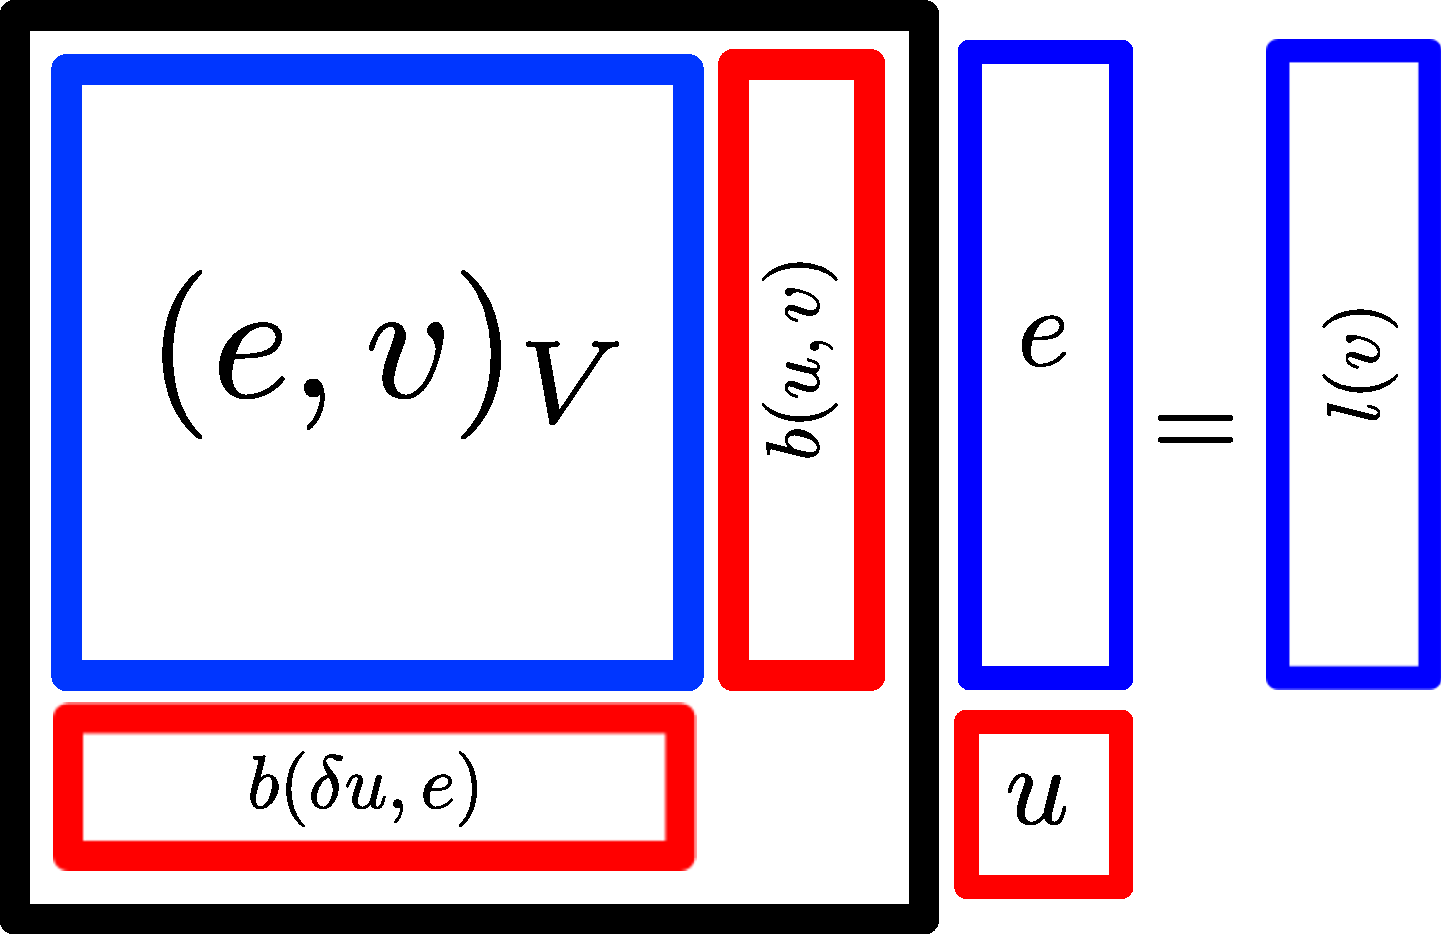
\includegraphics[scale=.3]{figs/saddlePoint.pdf}
%\caption{Saddle point system for minimization of $J(u_h)$; the Schur complement eliminating degrees of freedom for $e$ returns the system resulting from optimal test functions.}
%\end{figure}

This formulation was first introduced by Cohen, Dahmen, and Welper in \cite{DahmenVariationalStabilization}, where $V_h$ was determined adaptively.  The method proceeded in two steps -- first, $V_h$ was set equal to $U_h$ on what we will define as the \textit{coarse mesh}.  Next, \textit{a posteriori} error estimators for $e$ (based on a specific choice of inner product $\LRp{\cdot,\cdot}_V$) were used to drive adaptivity to determine a fine-scale mesh on which $V_h$ was supported.  We choose a simpler representation -- if $U_h$ is represented by piecewise polynomials of order $p$, we set $V_h$ to be piecewise polynomials of order $p+\triangle p$.  We note that these two choices of discretization for $V$ are not mutually exclusive, and that novel choices for $V_h$ are likely the key to yielding computationally effective methods under this framework.  
\subsection{DPG optimal test function framework}

The DPG method was introduced by Demkowicz and Gopalakrishnan in 2009, and rapidly applied to a series of problems in computational mechanics \cite{DPG2,DPG3,DPG4,maxwellDPG,stokesDPG}.  Though the DPG method shares the same variational setting as Cohen et al.\, each method followed very different approaches in implementation.  Recall the orthogonality of error~\eqref{rieszOrthog}; by defining the error representation function $e$ and undoing the Riesz map acting on $B\delta u$, we recovered a saddle point formulation.  However, it is possible instead to undo the Riesz map acting on the residual, to recover
\begin{align*}
\LRp{R_V^{-1}\LRp{l-Bu_h},R_V^{-1}B\delta u}_V &= 0, \quad \forall \delta u \in U_h\\
\Rightarrow \LRa{\LRp{l-Bu_h},R_V^{-1}B\delta u}_{V^*\times V} &= 0\\
\Rightarrow l\LRp{R_V^{-1}B\delta u}-b\LRp{u_h,R_V^{-1}B\delta u} &= 0
\end{align*}
If we define $v_{\delta u} \coloneqq R_V^{-1}B\delta u$, then we recover the original variational formulation with a nonstandard test space
\[
b(u_h,v_{\delta u}) = l(v_{\delta u}), \quad \forall \delta u \in U_h.
\]
The DPG method with optimal test functions was constructed under this perspective of minimization of $J(u_h)$.  While $v_{\delta u} \in V$ must still be solved for approximately, under the assumption of discontinuous test functions, this solve can be localized to a single element.\footnote{In practice, if $U_h(K) = P^p(K)$ is the space of polynomials of order $p$ over the element $K$, then the enriched space $V_h \subset V$ is chosen to be $V_h(K) = P^{p+\triangle p}(K)$, where $\triangle p \geq n$, and $d$ is the spatial dimension.}

We can draw yet another connection to the DPG method by considering the discrete problem which arises from the saddle point formulation.  Defining the vectors of coefficients $\bs{u} = \LRc{u_j}_{j=1}^{\dim{U_h}}$ and $\bs{e} = \LRc{e_j}_{j=1}^{\dim{V_h}}$, our discrete saddle point system is
\[
\left[\begin{array}{cc} \bs{A} &\bs{B}\\ \bs{B}^T&{0}\end{array}\right]\left[\begin{array}{c}\bs{e}\\ \bs{u}\end{array}\right] = \left[\begin{array}{c}\bs{f}\\ 0\end{array}\right],
\]
where, for basis functions $\psi_j\in U_h$ and $\phi_i,\phi_j\in V_h$, 
\[
\bs{A}_{ij} \coloneqq \LRp{\phi_i,\phi_j}_V, \quad \bs{B}_{ij} \coloneqq b\LRp{\psi_j,\phi_i},
\]
such that $\bs{A}$ is a square matrix and $\bs{B}$ is an overdetermined rectangular matrix.  Expressing $\bs{e} = \bs{A}^{-1}\LRp{\bs{f}-\bs{B}\bs{u}}$ allows us to statically condense out the degrees of freedom $\bs{e}$ to form the Schur complement
\[
\bs{B}^T \bs{A}^{-1}\bs{B} \bs{u} = \bs{B}^T \bs{A}^{-1}\bs{f}.
\]
The above system is essentially an algebraic least squares system, but preconditioned on the inside with the positive-definite operator $\bs{A}$, which is precisely the discrete system that arises under the optimal test function framework of DPG.  We can see this further by noting that 
\[
\LRp{\bs{A}^{-1}\bs{B}}^T\bs{B} \bs{u} = \LRp{\bs{A}^{-1}\bs{B}}^T\bs{f} 
\]
is equivalent to 
\[
b\LRp{u_h, \sum_k^{\dim{V_h}} v_{ik}\phi_k} = l\LRp{\sum_k^{\dim{V_h}} v_{ik}\phi_k}, \quad i = 1,\ldots,\dim(U_h)
\]
where $v_{ik} = \LRp{\bs{A}^{-1}\bs{B}}_{ik}$ are the degrees of freedom associated with the $i$th approximated optimal test function.

The efficiency of the DPG method lies in that, under the assumption of a localizable norm and optimal test functions, $\bs{A}$ is block diagonal and can be inverted locally \cite{overviewDPG}.  Under the ultra-weak formulation of DPG, one can show that this corresponds exactly to choosing a non-conforming DG space for $V$, where continuity is enforced weakly at element interfaces by requiring that the jump be orthogonal to polynomials of order $p$ \cite{globalLocalDPG}.\footnote{Such a weakly conforming method was first introduced in \cite{brenner2008mathematical}, where optimal rates of convergence were proved under the assumption that the DG space is at most of order $p+1$ .}  

\subsection{Variational Multiscale Framework}

The above saddle point system can also be directly derived from variational multiscale (VMS) principles \cite{VMS1,VMS2}.  The key difference between this and standard multiscale methods is the way in which the fine scales influence the coarse; approximating the fine-scale problem is as difficult as approximating the original equation, so analytic approximations or assumptions must typically be made.  However, through the proper change of variables, this method converts the fine-scale problem into a symmetric-positive definite one, allowing for a well-behaved subgrid model of fine scale behavior.

We begin again with the variational problem
\[
\LRa{Bu,v}_{V^*\times V} = \LRa{l,v}_{V^*\times V},
\]
where, as before, $B: U\rightarrow V^*$ is the operator form of $b(u,v)$, and $l \in V^*$ is the load.  Standard VMS techniques then decompose $U$ into a \textit{coarse scale} space $U_h$ and \textit{fine scale} space $U'$, such that the coarse and fine scales $u_h \in U_h \subset U$ and $u' \in U'$ are related through some yet-unspecified orthogonality condition.  Decomposing $u = u_h + u'$ gives 
\begin{align*}
u_h \in U_h, u' \in U', v \in V\\
\LRa{Bu_h,v}_{V^*\times V} + \LRa{Bu',v}_{V^*\times V} = \LRa{l,v}_{V^*\times V}
\end{align*}
where $U = U_h\oplus U'$.  We can now explicitly choose our orthogonality condition defining the fine scales and rewrite the above problem as 
\begin{align*}
u_h \in U_h, u' \in U, v \in V\\
\LRa{Bu_h,v}_{V^*\times V} + \LRa{Bu',v}_{V^*\times V} &= \LRa{l,v}_{V^*\times V}\\
\LRp{u',\bar{w}}_E &= 0, \quad \forall \bar{w} \in U_h,
\end{align*}
where $\LRp{u',\bar{w}}_E$ is defined through
\begin{align*}
\LRp{u',\bar{w}}_E = \LRp{Tu',T\bar{w}}_V\\
T:U\rightarrow V, \quad T \coloneqq R_V^{-1} B
\end{align*}
where $\LRp{v,\delta v}_V$ is an inner product on $V$ and $R_V$ is the Riesz map associated with this inner product.  DPG literature refers to $T$ as the \textit{trial-to-test} operator, which, given a basis function $\phi_i \in U_h$, returns the optimal test function for $\phi_i$ \cite{DPG2}.  

If we define our fine-scale using the above orthogonality condition, we have that
\begin{align*}
\LRp{Tu',v}_V = \LRp{R_V^{-1}Bu',v}_V = \LRa{Bu',v}_{V^*\times V}\\
\LRp{u',\bar{w}}_E = \LRp{Tu',R_V^{-1}B\bar{w}}_V = \LRa{Tu',B\bar{w}}_{V\times V^*}
\end{align*}
and can now rewrite our above VMS formulation as 
\begin{align*}
u_h \in U_h, u' \in U, v \in V\\
\LRa{Bu_h,v}_{V^*\times V} + \LRp{Tu',v}_{V} &= \LRa{l,v}_{V^*\times V}\\
\LRp{Tu',B\bar{w}}_{V\times V^*} &= 0, \quad \forall \bar{w} \in U_h.
\end{align*}
The saddle point formulation of Section~\ref{sec:saddlePoint} can be interpreted as solving not for $u'$, but for $e\coloneqq Tu'$.  The discrete approximation then follows directly from setting $V \coloneqq V_h$, some finite-dimensional enriched space, which impacts the method through the approximation of $Tu'$ via approximation of the Riesz map $R_V^{-1}$.  

To summarize, the minimum-residual framework motivating both Cohen, Dahmen, and Welper's variational stabilization and Demkowicz and Gopalakrishnan's DPG method can be characterized as a VMS method under which 
\begin{itemize}
\item Orthogonality of $U_h$ and $U'$ is defined through a nonstandard \textit{energy inner product} $$\LRp{u',\delta u}_E = 0, \quad\forall \delta u \in U_h,$$ 
\item A change of variables (i.\ e.\ solving for $Tu'$ instead of $u'$) symmetrizes the fine-scale contribution and overall system.
\end{itemize}

\section{Choices for test norms}

As with the DPG method, the primary theoretical difficulty is in defining the norm $\nor{v}_V$ such that the method returns good results.  This choice of norm defines the measure of the residual which we minimize or the orthogonality condition defining the separation of coarse and fine scales, depending upon whether you adopt the minimum-residual or VMS perspective.  

From this point on, we will focus specifically on $H^1$ standard Galerkin formulation for the scalar convection-diffusion problem on domain $\Omega$
\[
\div(\beta u) - \epsilon \del u = f,
\]
which represents the convection of some quantity $u$ subject to a convection field $\beta \in R^n$ and diffusion of magnitude $\epsilon \in \mbb{R}$, where $\epsilon > 0$.  We impose inflow and outflow boundary conditions
\begin{align*}
\left.u\right|_{\Gamma_{\rm in}} &= u_{\rm in}\\
\left.u\right|_{\Gamma_{\rm out}} &= u_{\rm out}
\end{align*}
where the following boundaries are defined as 
\begin{align*}
\Gamma_{\rm in}\coloneqq \LRc{x\in \partial \Omega:  \beta\cdot\vec{n}(x) \leq 0}\\
\Gamma_{\rm out}\coloneqq \LRc{x\in \partial \Omega: \beta\cdot\vec{n}(x) > 0}
\end{align*}
where $\vec{n}(x)$ is the outward normal at a point on the boundary $\partial \Omega$.  If it is non-empty, we may also define $\Gamma_{0}\coloneqq \LRc{x\in \partial \Omega s.\ t.\ \beta\cdot\vec{n}(x) = 0}$ as the boundary with outward normal orthogonal to the streamline.  For the remainder of this paper, we treat non-homogeneous boundary conditions as lifted forcing data, and consider only the homogeneous case.  

For $u\in H^1_0(\Omega)$, our weak formulation becomes
\[
\LRp{\Grad u,\beta v + \epsilon \Grad v}_{\L} = \LRp{f,v}_{\L}, \quad \forall v \in H^1_0.
\]
A norm based on the symmetric part of the bilinear form was explored in \cite{DahmenVariationalStabilization}, but yielded approximations which degnerated in $\epsilon$.  We present here two different methods based on alternative choices for test norms on $V$ for the convection-diffusion equation that both yield good results as $\epsilon\rightarrow 0$.  

We note that the first-order term $\LRp{\Grad u,\beta v}$ may also be integrated by parts.  The two are equivalent for $\div \beta = 0$ and give nearly identical results.

\subsection{Weighted streamline diffusion norm}

Our first method is motivated by previous results for the DPG method in \cite{DPGrobustness}, which achieved good results through a modification of the test norm.  We set
\[
\nor{v}_{V,w}^2 \coloneqq \frac{L}{\LRb{\beta}}\nor{\sqrt{w}\beta\cdot \Grad v}_{\L}^2 + \epsilon\nor{\Grad v}_{\L}^2 + \alpha\nor{v}_{\L}^2,
\]
where $L = \LRb{\Omega}^{\frac{1}{d}}$ is the length measure of $\Omega$ in $d$ spatial dimensions, $\LRb{\beta} = \max_\Omega \nor{\beta}_{l^2}$, and we have introduced the scaling $\frac{L}{\LRb{\beta}}$ on the streamline diffusion term for unit consistency\footnote{In all problems considered, $\frac{L}{\LRb{\beta}} = O(1)$.}. $\alpha \geq 0$ is a user-specified constant with units of inverse time\footnote{In the case where $\alpha = 0$, the seminorm remains a norm due to equivalence with the $H^1$ seminorm, which is norm on $H^1_0$.  Specifying $\alpha > 0$ does not change the results dramatically; however, it does appear to improve conditioning of $\bs{A}$.}, and $w(x)$ is some smoothly varying positive weighting function.  Specifically, we require $\LRb{w(x)}$ to be of magnitude $O(\epsilon)$ for $x\in \Gamma_{\rm in}$, but $O(1)$ away from the inflow boundary.\footnote{Specific restrictions on $w$ are derived in \cite{DPGrobustness} in context of the DPG method.}

A second motivation behind the weighting function can also be found in \cite{stynesSUPG, roos2008robust, johnsonCrosswind}, which refer to $w(x)$ as a cut-off function.  A theoretical issue with the convection-diffusion problem is that $\nor{u}_{H^1_0}$ and $\nor{u-u_h}_{H^1_0}$ do not remain bounded as $\epsilon\rightarrow 0$, due to the fact that $u' = O(\epsilon^{-1})$ in the region of boundary or internal layers.  These cut-off functions were introduced in order to yield $\epsilon$-independent bounds on the error by localizing error estimates away from layers.

We can demonstrate the need for the weight/cut-off function $w(x)$ in the test norm -- Figure~\ref{fig:comparison1D} shows the result of two simulations on a uniform 16 element piecewise-linear mesh. The error representation $e$ is approximated by quadratics over the same mesh.  Without the weight, the solution degenerates near the inflow; a similar phenomenon was observed in \cite{DahmenVariationalStabilization, DPG2, globalLocalDPG}.  
\begin{figure}[!h]
\centering
\subfigure[Solution $u$]{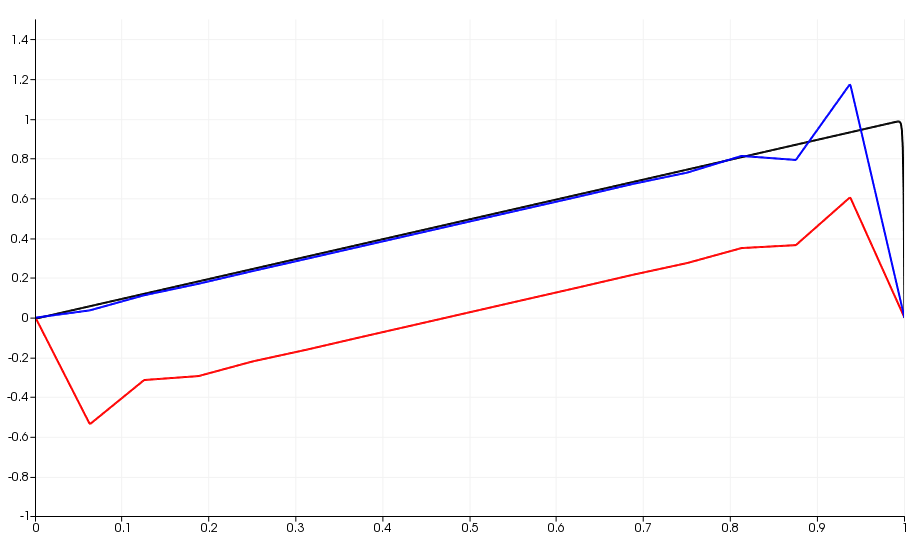
\includegraphics[scale=.22]{figs/weightedComparison1D.png}}
\subfigure[Fine-scales $e$]{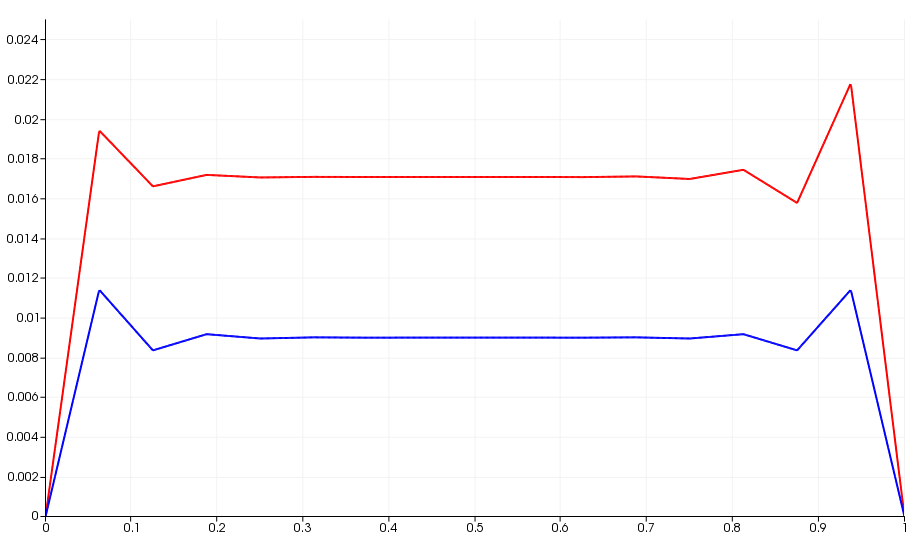
\includegraphics[scale=.22]{figs/weightedErrorComparison1D.png}}
\caption{Comparisons of $u$ and $e$ for $\epsilon = 10^{-3}$, $f=1$ and $\alpha = 0$. The solution when $w = 1$ is in red, and the solution for when $w = x+\epsilon$ is given in blue.  The exact solution is given in black.}
\label{fig:comparison1D}
\end{figure}

Physically speaking, the weight can be interpreted as a cutoff function for the adjoint solution \cite{DPGrobustness2}, which displays a boundary layer at the inflow due to the fact that the direction of convection is reversed for the adjoint equation.  Mathematically speaking, it can also be interpreted as restoring a sense of directionality to the test norm (which is  sign of $\beta$).  

\subsection{Streamline norm with weak boundary conditions on $e$}

While the above norm appears to give improved results, the issue of constructing a weighting function for complex geometries in higher dimensions can be fairly nontrivial.  One possibility would be to solve a Laplace's equation for $w$ on the domain, enforcing that $w(x) = \epsilon$ at inflow boundaries; however, the behavior of such a computationally determined weight has not been examined, and incurs additional complexity that is avoided by other methods.  

Under this saddle-point framework, however, it is possible to avoid the use of a weight altogether.  Currently, we seek $v,e\in H^1_0(\Omega)$; however, if we seek instead 
\[
v,e\in H^1_{\rm out}(\Omega) \coloneqq \LRc{v\in H^1(\Omega) s.\ t.\ \left.v\right|_{\Gamma_{out}} = 0},
\]
we modify our variational formulation to be
\[
\LRp{\Grad u,\beta v + \epsilon \Grad v}_{\L} - \epsilon\int_{\Gamma_{\rm in}} \pd{u}{n}v = \LRp{f,v}_{\L}.
\]
Under this modification of the variational formulation, we can set $w=1$ and use the test norm
\[
\nor{v}_{V}^2 \coloneqq \frac{L}{\LRb{\beta}}\nor{\beta\cdot \Grad v}_{\L}^2 + \epsilon\nor{\Grad v}_{\L}^2 + \alpha\nor{v}_{\L}^2
\]
without experiencing the issues displayed for $e\in H^1_0(\Omega)$ in Figure~\ref{fig:comparison1D}.  

Physically speaking, the replacement of $H^1_0(\Omega)$ with $H^1_{\rm out}(\Omega)$ can be viewed as releasing the strong imposition of a boundary condition at the inflow.  
%If $\alpha > 0$, then $\nor{v}_V^2$ defines an inner product $H^1(\Omega)$ and can be inverted without the application of boundary conditions.  If we ignore regularity restrictions on $u$ momentarily, the inversion of $\LRp{e,v}_V$ over $H^1_{\rm out}$ then corresponds to the strong problem
%\begin{align*}
%\alpha e - \Div \LRp{\LRp{\beta \otimes \beta + \epsilon I}\Grad e} &= f- \LRp{\beta\cdot \Grad u - \epsilon \del u}\\
%\vec{n}\cdot \LRp{\beta \otimes \beta + \epsilon I} \Grad e - \epsilon \vec{n}\cdot\Grad u &= 0, \quad \text{on }\Gamma_{\rm in}\\
%e &= 0, \quad \text{on }\Gamma_{\rm out}
%\end{align*}
%In other words, the Dirichlet boundary condition at $\Gamma_{\rm in}$ is replaced by a stress boundary condition, releasing the presence of a boundary layer at the inflow.  
The addition of the term $\epsilon\int_{\Gamma_{\rm in}} \pd{u}{n}v$ is akin to a penalty term that weakly enforces a homogeneous boundary condition on $e$ at the inflow; the orthogonality condition for $e$ under this additional term is
\[
(\Grad \delta u, \beta e + \epsilon \Grad e)_{\L} - \epsilon\int_{\Gamma_{\rm in}} \pd{\delta u}{n}e = 0, \quad \forall \delta u \in U_h
\]
If $U_h$ is taken to be a polynomial space of order $p$, the first term enforces orthogonality of $\beta e + \epsilon \Grad e$ to polynomials of order $p-1$ on the interior, while the second term enforces orthogonality of $e$ to polynomials of order $p-1$ on the subset of the boundary $\Gamma_{\rm in}$.  %If $e$ is represented by a polynomial of order $p-1$, then this condition reduces to strong enforcement of $\left. e\right|_{\Gamma_{\rm in}}=0$ \cite{brenner2008mathematical}.  
This boundary condition is released in the limit as $\epsilon \rightarrow 0$; as a result, for small $\epsilon$, the contribution $\LRp{e,v}_V$ no longer provides extraneous stabilization at the inflow for under-resolved meshes.  However, for large $\epsilon$, the boundary condition activates and $e$ recovers homogeneous boundary conditions over the entire space $V$.  The choice of weight $w(x)$ in the previous section can be seen as similarly removing the contribution of $e$ near the inflow for small $\epsilon$, but allowing it to return for large $\epsilon$.  

A comparison between the weighted norm $\nor{v}_{V,w}$ with $e\in H^1_0(\Omega)$ and unweighted norm with $e\in H^1_{\rm out}$ in one dimension is given in Figure~\ref{fig:robustComparison1D}.   We note that Broersen and Stevenson have also achieved good results by making use of the space $H^1_{\rm out}(\Omega)$ in their application of the DPG method to the mixed mild-weak formulation for convection-diffusion \cite{broersenStevenson}.
\begin{figure}[!h]
\centering
\subfigure[Solution $u$]{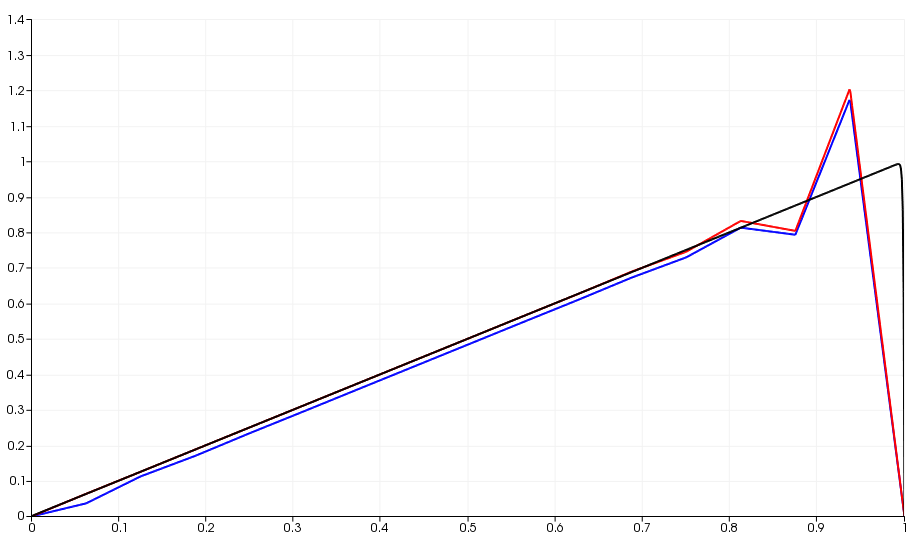
\includegraphics[scale=.22]{figs/robustComparison1D.png}}
\subfigure[Fine-scales $e$]{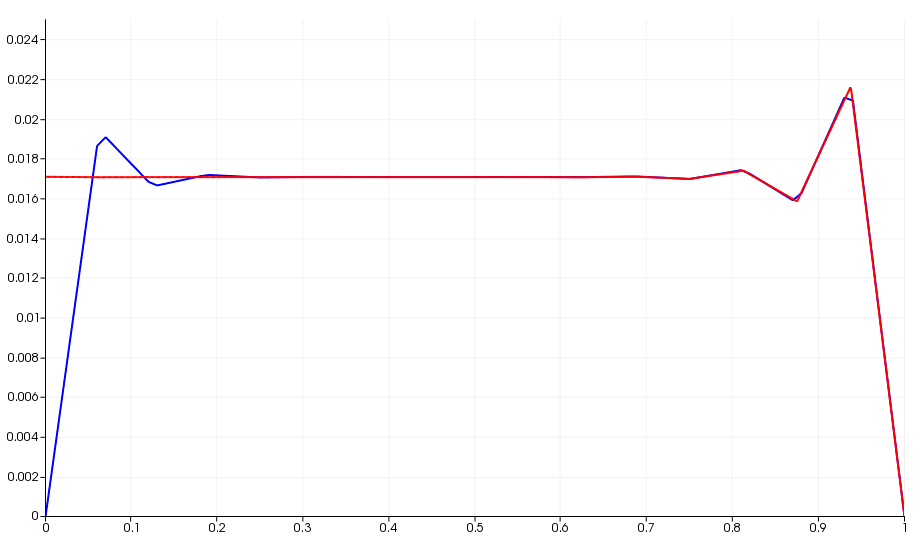
\includegraphics[scale=.22]{figs/robustErrorComparison1D.png}}
\caption{Comparisons of $u$ and $e$ for $\epsilon = 10^{-3}$, $f=1$ and $\alpha = 0$. The solution when $w = 1$ and $e\in H^1_{\rm out}(\Omega)$ is in red, and the solution for when $w = x+\epsilon$ is given in blue.  The exact solution is given in black.}
\label{fig:robustComparison1D}
\end{figure}

\begin{remark}
We remark that this inclusion of $\epsilon\int_{\Gamma_{\rm in}} \pd{u}{n}v$ is a variational crime under the assumption that $u \in H^1_0(\Omega)$; the proper way to include such a term in a conforming manner (without introducing additional regularity assumptions on $u$) would be to introduce $\epsilon \pd{u}{n}$ as an additional unknown on the boundary, similar to the work done using DPG under the ultra-weak formulation \cite{DPG2,analysisDPG}.  However, we have found that doing so does not remove the boundary layer in the residual at the inflow, and numerical results appear to degenerate in quality as $\epsilon$ grows smaller and smaller.  We believe this is due to the fact that, by identifying $\epsilon \pd{u}{n}$ as an additional unknown, the orthogonality boundary condition $\int_{\Gamma_{\rm in}} \pd{u}{n} e = 0$ is decoupled from the interior integrals and enforced strongly.  The same situation occurs when $\pd{u}{n}$ is declared as an additional unknown and when $\epsilon > 0$.  %The mild-weak formulation effectively enforces the orthogonality of $e$ to polynomials of lower order on $\Gamma_{\rm in}$ in a conforming manner, by introducing an additional flux unknown representing $\epsilon \pd{u}{n}$.  

%For many flow problems, activity near the inflow is typically very smooth and can thus be represented using a minimal number of elements under an effective adaptive mesh refinement scheme, implying that the cost of introducing such additional unknowns on $\Gamma_{\rm in}$ can be minimized.  However, since the codebase we currently use does not feature unknowns with support only on element edges/faces, we continue to operate under this variational crime, in hopes that we can implement a conforming version in the near future.  %Another way to properly include the term $\epsilon \pd{u}{n}$ in the variational formulation would be to work with higher continuity trial spaces that admit a normal trace of the derivative on the boundary \cite{nurbsTrace, NURBSorig}.  
\end{remark}
\begin{remark}
Various other methods of implementing a weak boundary condition on $e$ at the inflow $\Gamma_{\rm in}$ were implemented; for example, the inner product $\LRp{e,v}_V$ was modified by adding the a weak penalization term $$\epsilon C(h,p+\triangle p)\int_{\Gamma_{\rm in}}ev $$ to enforce the boundary condition at $\left.e\right |_{\Gamma_{\rm in}}$, where $C(h,p+\triangle p) = p^2/h$, which is a common choice of penalization parameter in high order finite element literature \cite{nurbsTrace,Warburton20032765}. However, the inclusion of the nonconforming term $\epsilon\int_{\Gamma_{\rm in}} \pd{u}{n}v$ in the bilinear form still resulted in the best solutions for all our numerical tests.  
\end{remark}

%\subset H^1_0(\Omega) \cap \LRc{w\in H^{\frac{3}{2}+\delta}(\Omega): \left.\pd{w}{n}\right|_{\Gamma_{\rm in}} \in H^{\frac{1}{2}}(\Gamma_{\rm in})}
Thus, the full formal characterization of the second method can be given as follows - solve for $u\in U_h \subset H^1_0(\Omega)\cap H^{\frac{3}{2}+\delta}(\Omega)$ (where $\delta$ is an positive real number), $e\in V_h\subset H^1_{\rm out}(\Omega)$ such that
\begin{align*}
\LRp{e,v}_V + (\Grad u, \beta v + \epsilon \Grad v)_{\L} - \epsilon\int_{\Gamma_{\rm in}} \pd{u}{n}v &= (f,v)_{\L}, \quad \forall v \in V_h\\
(\Grad \delta u, \beta e + \epsilon \Grad e)_{\L} - \epsilon\int_{\Gamma_{\rm in}} \pd{\delta u}{n}e &= 0, \quad \forall \delta u \in U_h
\end{align*}
where
\begin{align*}
\LRp{e,v}_V \coloneqq \LRp{\beta\cdot \Grad e,\beta\cdot \Grad v}_{\L} + \epsilon \LRp{\Grad e,\Grad v}_{\L}.
\end{align*}
We will utilize this second version of the method for all following numerical examples.  


\begin{remark}
We note that, when the Peclet number ${\rm Pe} = \frac{\LRb{\beta} L}{\epsilon} \gg 1$, the boundary term $\epsilon\int_{\Gamma_{\rm in}} \pd{u}{n}v$ effectively disappears, and numerically speaking, we can use $e,v\in H^1_{\rm out}(\Omega)$ without including the additional boundary term in the variational formulation.  
\end{remark}

\subsection{Stability theory}
While a full proof of stability has not yet been developed, Brezzi theory for mixed methods \cite{BabuskaEquivBrezzi} allows us to demonstrate stability on quasi-uniform meshes for under-resolved regimes.  
\begin{lemma}
Assume the following conditions hold
\begin{enumerate}
\item $V_h$ is sufficiently ``rich'', such that, for some $\gamma > 0$, 
$$\nor{\Pi_{V_h}\LRp{\beta\cdot \grad\delta u}}_{\L} \geq \gamma \nor{\beta\cdot \grad\delta u}_{\L},\quad \forall \delta u\in U_h,$$
where $\Pi_{V_h}$ is the $L^2$-orthogonal projection onto $V_h$.  
\item The convection field $\beta$ satisfies $\div \beta = 0$ and
\[
\beta\cdot \grad \psi \geq b_0 > 0, \quad {\rm in} \Omega
\]
for some $\psi\in C^1(\bar{\Omega})$.
\item $\sqrt{\epsilon} \ll h$, where $h$ is the mesh size.
\end{enumerate}
Under these assumptions, we can prove quasi-optimality of the method in the $L^2$-norm.
\[
\nor{u-u_h}_{\L} + \nor{e-e_h}_{\L} \leq C_h \inf_{w_u\in U_h, w_e\in V_h}\LRp{\nor{u-w_u}_{\L} + \nor{e-w_e}_{\L}}
\]
\end{lemma}
\begin{proof}
The result follows from proving two conditions in Brezzi theory; the first condition (inf-sup in the kernel) reduces to the coercivity condition
\begin{equation}
\LRp{e,v}_V = \epsilon\LRp{\grad e,\grad v}_{\L} + \LRp{\beta\cdot\grad e,\beta\cdot \grad v}_{\L} \geq C_1\nor{v}_{\L},\quad \forall v\in V_h,
\label{eq:cond1}
\end{equation}
while the second condition is 
\begin{equation}
\sup_{v\in V_h\setminus \{0\}} \frac{b(u,v)}{\nor{v}_{L^2}} = \frac{ (\Grad u, \beta v + \epsilon \Grad v)_{\L} - \epsilon\int_{\Gamma_{\rm in}} \pd{u}{n}v}{\nor{v}_{L^2}} \geq C_2\nor{u}_{L^2}. 
\label{eq:cond2}
\end{equation}
The first condition \ref{eq:cond1} can be proven by noticing that 
\[
\nor{\beta\cdot\grad v}_{\L} = \sup_{w\in \L\setminus\{0\}}\frac{\LRp{\beta\cdot\grad v,w}_{\L}}{\nor{w}_{\L}}.
\]
We take $w = -e^{\psi}v$, noting that $\div \LRp{\beta w} \geq \div\beta e^\psi v + b_0 e^\psi v +  e^\psi \beta\cdot \grad v$.  Integrating by parts and rearranging, we recover
\begin{align*}
2\LRp{\beta\cdot\grad v,w}_{\L} &\geq \int_{\Gamma_{\rm in}} - \beta_n v^2e^\psi + \LRp{v,\div \beta e^\psi v + b_0 \psi e^\psi v}_{\L} \\
&\geq \LRp{v,b_0 e^\psi v}_{\L}.
\end{align*}
by $\beta_n < 0$ on $\Gamma_{\rm in}$ and Assumption 2.  Since $\psi$ is determined up to a constant, we set the constant such that $e^\psi = O(1)$ to arrive at the result.%; an application of Assumption 1 then gives~\ref{eq:cond1}. \textcolor{red}{How does Assumption 1 help?}

To prove~\ref{eq:cond2}, we first take $v = \Pi_{V_h}(\beta\cdot \grad u_h)$ for arbitrary $u_h\in U_h$.  Then, by Assumption 1,
\[
(\beta \grad u_h,v)_{\L} = \nor{\Pi_{V_h}\beta\cdot\grad u_h}_{\L}^2 \geq \gamma \nor{\beta\cdot\grad u_h}_{\L}^2.
\]
Since $u_h\in H^1_0$, by a similar argument in the proof of~\ref{eq:cond1}, we can show
\[
(\beta \grad u_h,v)_{\L} \geq \gamma \nor{\beta\cdot\grad u_h}_{\L}^2 \geq \bar{C}_2 \LRp{\nor{u_h}_{\L}^2 + \nor{\beta\cdot\grad u_h}_{\L}^2}.
\]
Finally, note that
\begin{align*}
\LRb{\epsilon (\Grad u_h, \Grad v)_{\L}} &\leq \epsilon \nor{\Grad u_h}_{\L}\nor{\Grad v}_{\L} \leq \epsilon h^{-2} \nor{u_h}_{\L}\nor{v}_{\L} \\
&\leq c_1 \nor{u_h}_{\L}\nor{v}_{\L},\\
\LRb{\epsilon\int_{\Gamma_{\rm in}} \pd{u_h}{n}v} &\leq  \epsilon h^{-2} \nor{u_h}_{\L}\nor{v}_{\L} \leq c_2\nor{u_h}_{\L}\nor{v}_{\L},
\end{align*}
using Assumption 3 and standard trace and inverse inequalities on quasi-uniform meshes.  Note that $\nor{v}_{\L} = \nor{\beta\cdot\grad u_h}_{\L}$; assuming $c_1$ and $c_2$ are sufficiently small relative to $\bar{C}_2$, an application of discrete Cauchy Schwarz gives 
\[
(\Grad u_h, \beta v + \epsilon \Grad v)_{\L} - \epsilon\int_{\Gamma_{\rm in}}\pd{u_h}{n}v \geq C_2 \LRp{\nor{u_h}^2_{\L} + \nor{\beta\cdot\grad u_h}^2_{\L}}
\]
which proves~\ref{eq:cond2}.
\end{proof}

\begin{remark}
Ideally, we would prove the above result under the stronger norm $\nor{v}_V$ for $v$ and a stronger norm on $u$.  Under the test norm on $V$, \ref{eq:cond1} would be satisfied trivially; however, we have not yet been able to prove \ref{eq:cond2} yet under a stronger norm on $v$.  
\end{remark}
\section{Numerical examples}

We present several numerical examples, demonstrating rates of convergence and performance of the method on several benchmark problems in 2D.  All numerical examples were executed using the %Python-based
 FEniCS codebase \cite{LoggMardalEtAl2012a} to demonstrate that, unlike previous methods based upon the minimization of dual residuals, this method is easily implemented in most standard high-order finite element codes.  

A remaining choice to be specified is the discretization of $V_h$: if $U_h$ is given to be polynomials of order $p$, the enriched space $V_h$ under which the fine-scales are approximated is set to be polynomials of order $p+\triangle p$ -- in other words, we use a simple polynomial enrichment scheme over a fixed mesh to approximate the fine-scale error representation function $e$.  In all experiments, $\triangle p = 1$ has been found to be sufficient, and larger $\triangle p$ has not been found to have a significant effect on the behavior of the method.  Table~\ref{tab:dp} shows the effect of increased $\triangle p$ on a uniform mesh; there is less than $.5\%$ change in $L^2$ error between $\triangle p = 1$ and $\triangle p=2$, and less than $.1\%$ change between $\triangle p=2$ and $\triangle p = 3$.\footnote{This is in contrast to the original DPG method, which also adopts a polynomial enriched space (where enrichment is done locally over each element) -- results by Gopalakrishnan and Qiu in \cite{practicalDPG} suggest that only $\triangle p \geq d$, where $d$ is spatial dimension, is guaranteed to yield optimal convergence rates for Laplace's equation. However, it is unknown if these results carry over to this new formulation.}

%Numerical experiments indicate that the measure of energy error is fairly insensitive to the degree of enrichment of $V_h$, so we expect that only a moderately finer resolution of $V_h$ with respect to $U_h$ is sufficient to capture fine-scale effects.  %More investigation is necessary to determine the nature of the energy norm induced by this method.  

\begin{figure}[!h]
\centering
  \begin{tabular}{| l || c | c | c | c| }
   \hline
    Order & Energy, $\epsilon=1$ & $L^2$, $\epsilon=1$  & Energy, $\epsilon=10^{-4}$ & $L^2$, $\epsilon=10^{-4}$\\
    \hline
    $\triangle p=1$ & 0.228580909 &  0.012003627 & 0.130406706 & 0.126763142
    \\ \hline
    $\triangle p=2$ &    0.230296524 &  0.011963812 & 0.130408851&    0.126763338
    \\ \hline
    $\triangle p=3$ &     0.230781435 & 0.011953146  &    0.130410190 &   0.126763389
    \\ \hline
    $\triangle p=4$ &    0.230900562 &  0.011950356 &   0.130410964 &  0.126763422
    \\ \hline
  \end{tabular}
\caption{Effect of $\triangle p$ on $L^2$ and energy error.}
\label{tab:dp}
\end{figure}

We report only $L^2$ errors for each example, due to the fact that $H^1$ error is not a well-defined quantity as $\epsilon \rightarrow 0$.  As a consequence, during adaptive refinement, the error does not always monotonically decrease or behave as expected, since adaptive refinement is driven by the the quantity $\nor{u-u_h}_E = \nor{e}_V$, which we expect to be equivalent (possibly with equivalence constants depending on $\epsilon$) to the $H^1$ norm.  We do expect $\nor{u-u_h}_E$ to decrease monotonically for all $\epsilon$ (though not uniformly in $\epsilon$) due to the minimum-residual nature of our method.  

\subsection{Erikkson-Johnson model problem}

We adopt a problem first proposed by Eriksson and Johnson in \cite{Eriksson1993} and later used in \cite{DPGrobustness, DPGrobustness2} to determine the robustness of the Discontinuous Petrov-Galerkin method with respect to the diffusion parameter $\epsilon$. For the choice of $\Omega = (0,1)^2$, $f=0$, and $\beta = (1,0)^T$, the convection diffusion equation reduces to
\[
\pd{u}{x} - \epsilon \left(\pdd{u}{x}+ \pdd{u}{y}\right) = 0,
\]
which has an exact solution by separation of variables, allowing us to analyze convergence of DPG for a wide range of $\epsilon$. For boundary conditions, we impose
\begin{align*}
u &= u_0, \quad x=0,\\
u &= 0, \quad x=1, y = 0,1
\end{align*}
In this case, our exact solution is the series
\[
u(x,y) = \sum_{n=0}^\infty C_n \frac{e^{r_{1,n}(x-1)} - e^{r_{2,n}(x-1)}}{e^{-r_{1,n}} - e^{-r_{2,n}}} \sin (n\pi y)
\]
where
\begin{align*}
r_{1,2,n} &= \frac{1 \pm \sqrt{1 + 4 \lambda_n}}{2 \epsilon},\\
\lambda_n &= n^2\pi^2 \epsilon.
\end{align*}
We choose boundary conditions such that the exact solution is given with $C_0 = 1$ and $C_n = 0$ for $n\neq 1$.  
\begin{align*}
u(x,y) &= \frac{e^{r_{1}(x-1)} - e^{r_{2}(x-1)}}{e^{-r_{1}} - e^{-r_{2}}} \sin (\pi y)\\
r_{1,2} &= \frac{1 \pm \sqrt{1 + 4 \epsilon^2 \pi^2}}{2 \epsilon},
\end{align*}
The problem is driven solely by inflow boundary conditions, and develops a boundary layer of width $\epsilon$ at the outflow $x = 1$.  
The resulting solution is shown in Figure~\ref{fig:erikkson} for $\epsilon = 10^{-2}$, along with convergence rates of $\L$ error under uniform mesh refinement for various $p$.  
\begin{figure}[!h]
\centering
\subfigure[Exact solution for $u$]{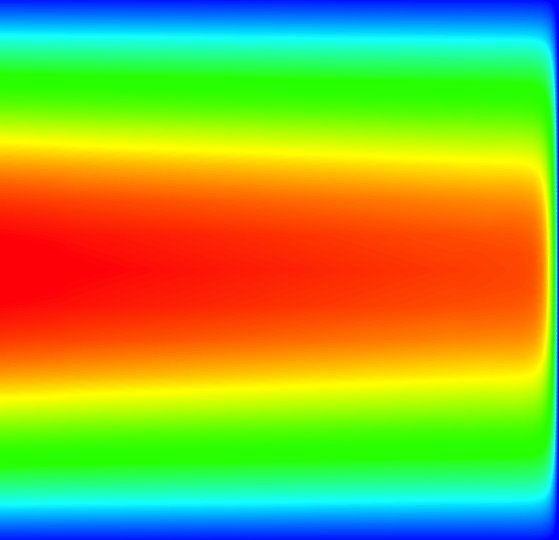
\includegraphics[width = .4\textwidth]{figs/erikksonExact.png}}
\subfigure[Convergence rates for $\epsilon = 10^{-2}$]{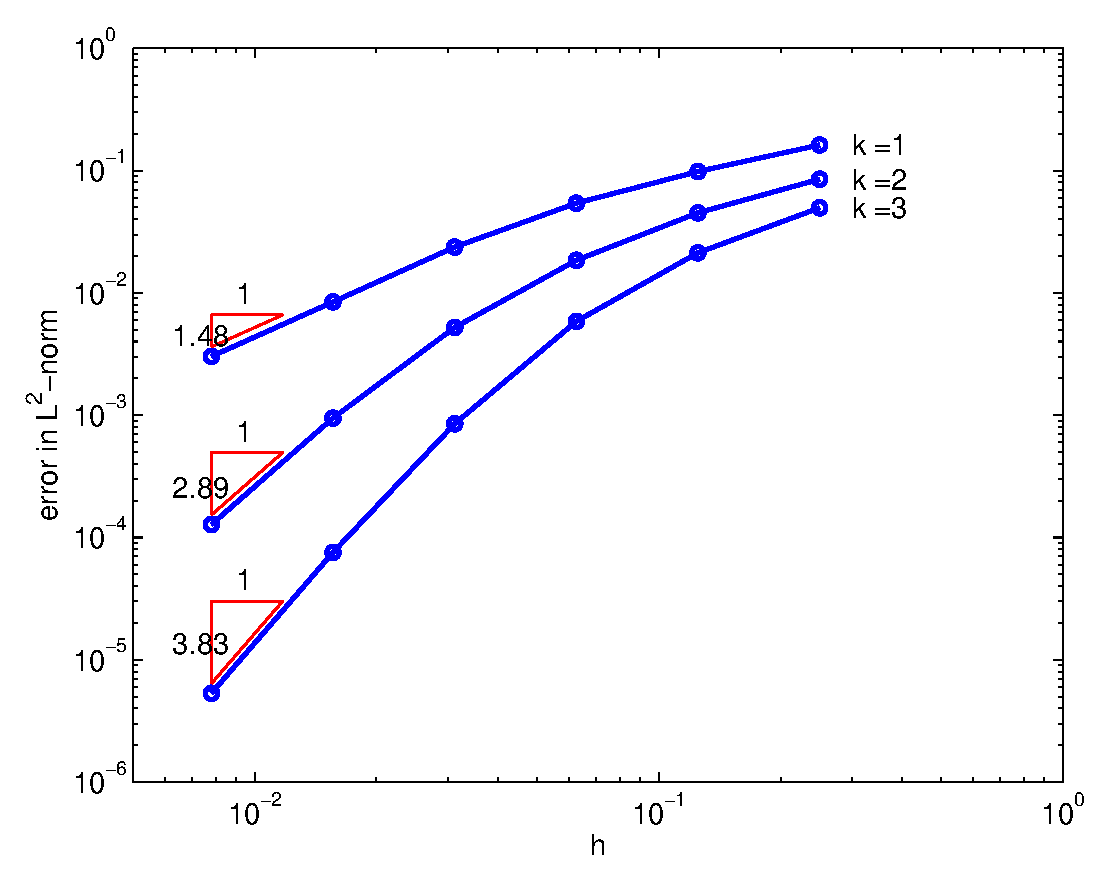
\includegraphics[width = .5\textwidth]{figs/rates/eps1e2Rates.eps}}
\caption{Erikkson-Johnson model problem for $\epsilon = 10^{-2}$, along with convergence rates under uniform refinement.}
\label{fig:erikkson}
\end{figure}

Optimal rates of convergence are not expected for small $\epsilon$ due to the pre-asymptotic nature of the mesh relative to the solution -- typically, $h$ must be $O(\epsilon)$ in order to observe optimal rates of convergence \cite{SchwabBoundaryLayers}.  

For large diffusion -- $\epsilon = 1.0$, we do observe optimal $p+1$ rates of convergence in Figure~\ref{fig:erikkson2}.  Likewise, when $\epsilon \ll h$, we observe a sub-optimal rate of $\frac{1}{2}$, the same as the rate suggested by theory and observed numerically in \cite{broersenStevenson} due to the strong boundary layer present under small diffusion.
\begin{figure}[!h]
\centering
\subfigure[$\epsilon = 1$]{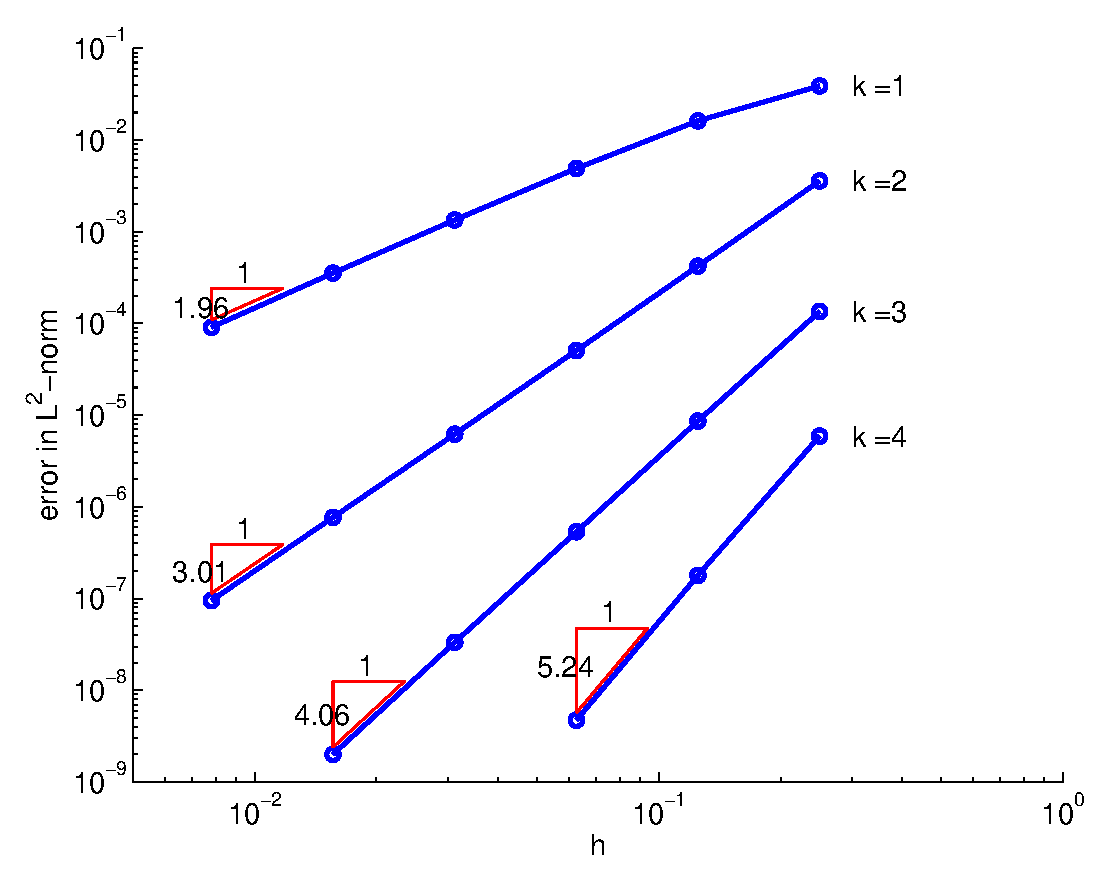
\includegraphics[width = .475\textwidth]{figs/rates/eps1e0Rates.eps}}
\subfigure[$\epsilon = 10^{-4}$]{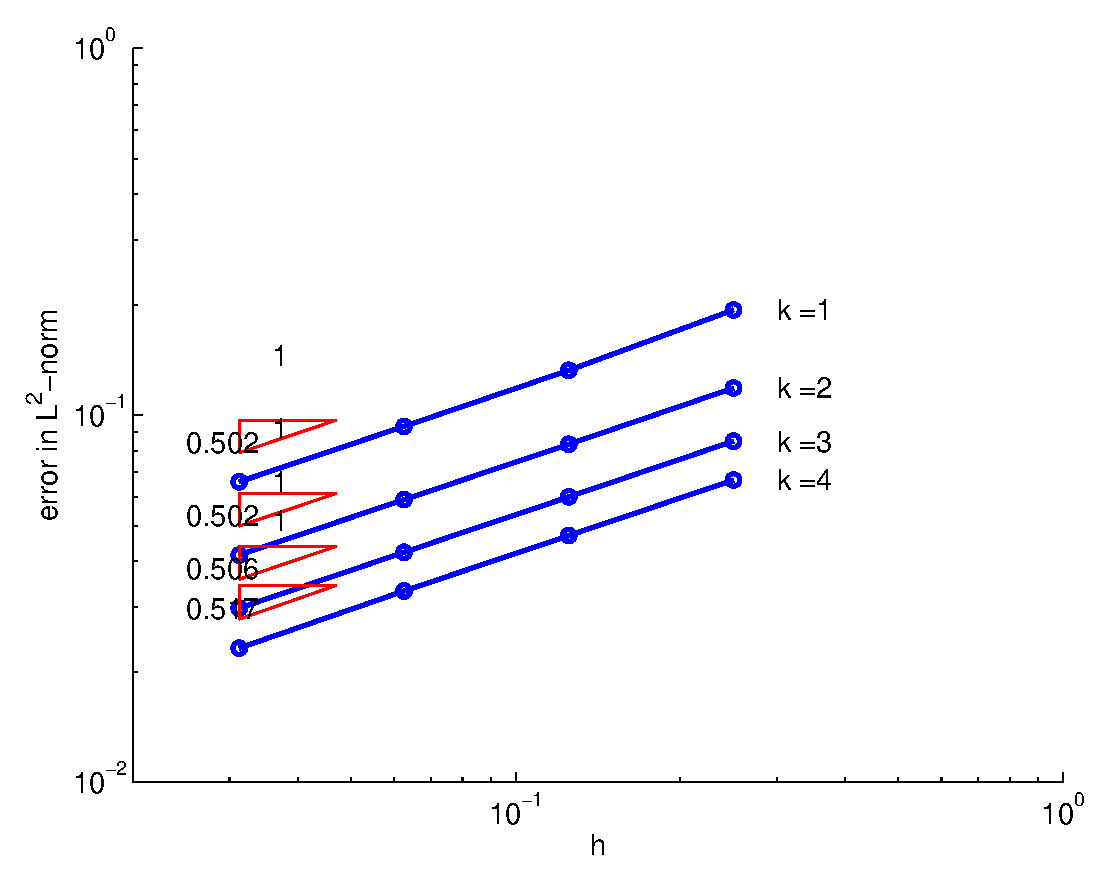
\includegraphics[width = .475\textwidth]{figs/rates/eps1e4Rates.eps}}
\caption{Erikkson-Johnson model problem for $\epsilon = 1$ and $\epsilon = 10^{-4}$, along with convergence rates under uniform refinement.}
\label{fig:erikkson2}
\end{figure}

\section{Adaptive mesh refinement}

We experimented also with an adaptive refinement scheme.  Since $\nor{e}_V$ is localizable\footnote{A localizable norm $\nor{v}_{V(\Omega)}$ can be written in the form 
$$\nor{v}_{V(\Omega)}^2 = \sum_{K\in \Oh} \nor{v}_{V(K)}^2,$$ where $\nor{v}_{V(K)}$ is a norm over each element $K$ in the mesh $\Oh$.}, we can evaluate it element-wise to get element error indicators $e_K \coloneqq \nor{e}_{V(K)}$.  We implemented a bulk-chasing refinement strategy, where, given some factor $\theta \in [0,1]$, we refine the top $\lceil{\theta N}\rceil$ elements with the largest error indicators $e_K$.  A greedy refinement scheme was also implemented, where all elements with $e_K > \theta \max_K e_K$ are refined; however, this refinement scheme tended to place refinements more conservatively, requiring many more refinement iterations to achieve a qualitatively good resolution.  In all following experiments, $\theta$ is set to be $.25$.  

\subsection{Erikkson-Johnson model problem}

We continue to verify our method using the Erikkson-Johnson with $\epsilon = 10^{-3}$.  The solution $u$ and the convergence/rates of $\L$ error under adaptive mesh refinement for $p=2$ are given in Figure~\ref{fig:erikksonAdapt}.  The energy error $\nor{u-u_h}_E$ is also displayed for comparison.  
\begin{figure}[!h]
\centering
\subfigure{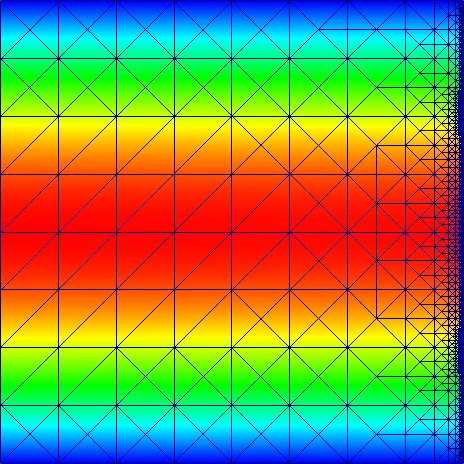
\includegraphics[width = .4\textwidth]{figs/erikkson1e3.png}}
\subfigure{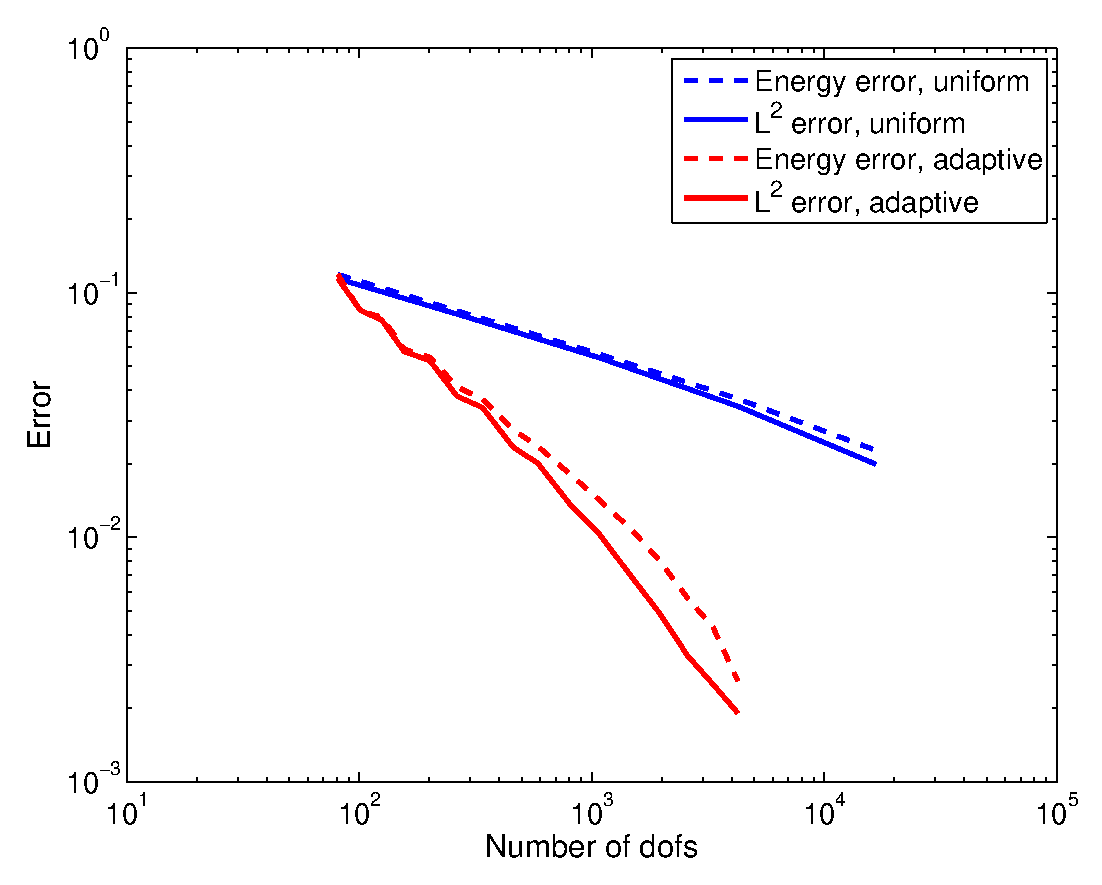
\includegraphics[width = .5\textwidth]{figs/rates/eps1e3Rates.eps}}
\caption{Erikkson-Johnson problem with $p = 2, \epsilon = 10^{-3}$ under 16 refinements.}
\label{fig:erikksonAdapt}
\end{figure}

We can also examine the fine-scale error representation function $e$.  Figure~\ref{fig:erikksonError} displays a comparison between the error representation function after the first iteration of adaptive mesh refinement and the 16th iteration.  Recall that the main contribution to the energy error is the streamline derivative of $e$; $\nor{u-u_h}_E^2 = \nor{e}_V^2 = \nor{\beta \cdot \Grad e}_{\L}^2 + \epsilon\nor{\Grad e}_{\L}^2$. Thus, variation in the streamline direction is picked up by $\nor{\beta\cdot \Grad e}_{\L}^2$ and is the primary contribution to the total error.  After sufficient refinement and resolution of the outflow layer, the error representation function becomes smooth in the region of the boundary layer, and refinements will be placed according to the viscous error $\epsilon\nor{\Grad e}_{\L}^2$. 

\begin{figure}[!h]
\centering
\subfigure{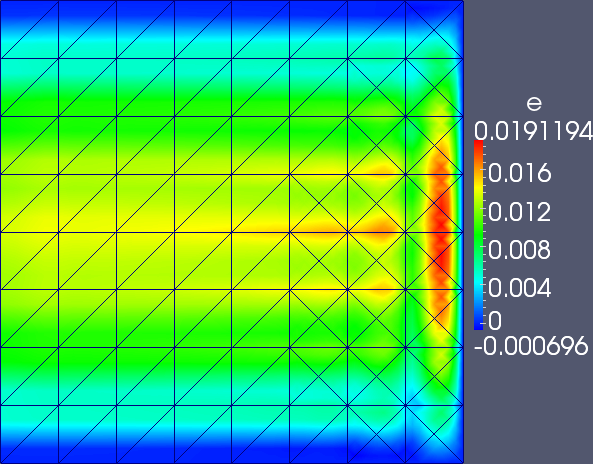
\includegraphics[width = .475\textwidth]{figs/erikkson1e3ErrUnif.png}}
\subfigure{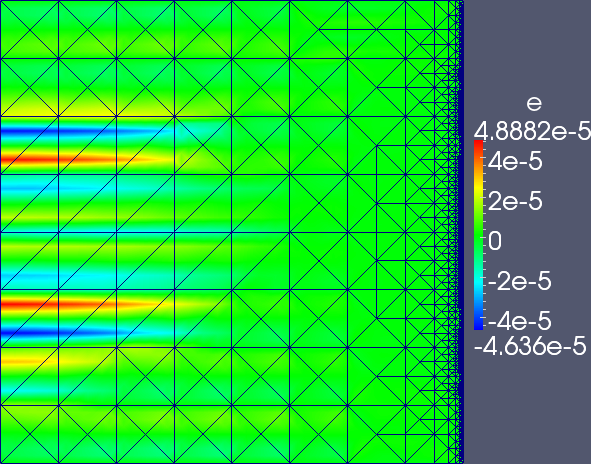
\includegraphics[width = .475\textwidth]{figs/erikkson1e3Err.png}}
\caption{Comparison of the fine scale error representation $e$ under the Erikkson-Johnson problem with $\epsilon = 10^{-3}$ for the mesh at the first and $16$th refinement steps.}
\label{fig:erikksonError}
\end{figure}

One open question concerning this method is the energy norm $\nor{u}_E$ which is induced by our choice of bilinear form and inner product on our choice of test space $V = H^1_{\rm out}$.  Figure~\ref{fig:erikksonEpsComparison} displays both $L^2$ and energy errors over a range of $\epsilon$.  We observe that the energy error appears to converge to the $L^2$ error as $\epsilon$ vanishes, however, for larger $\epsilon$, an explicit expression for the energy error has not yet been derived.  

\begin{figure}[!h]
\centering
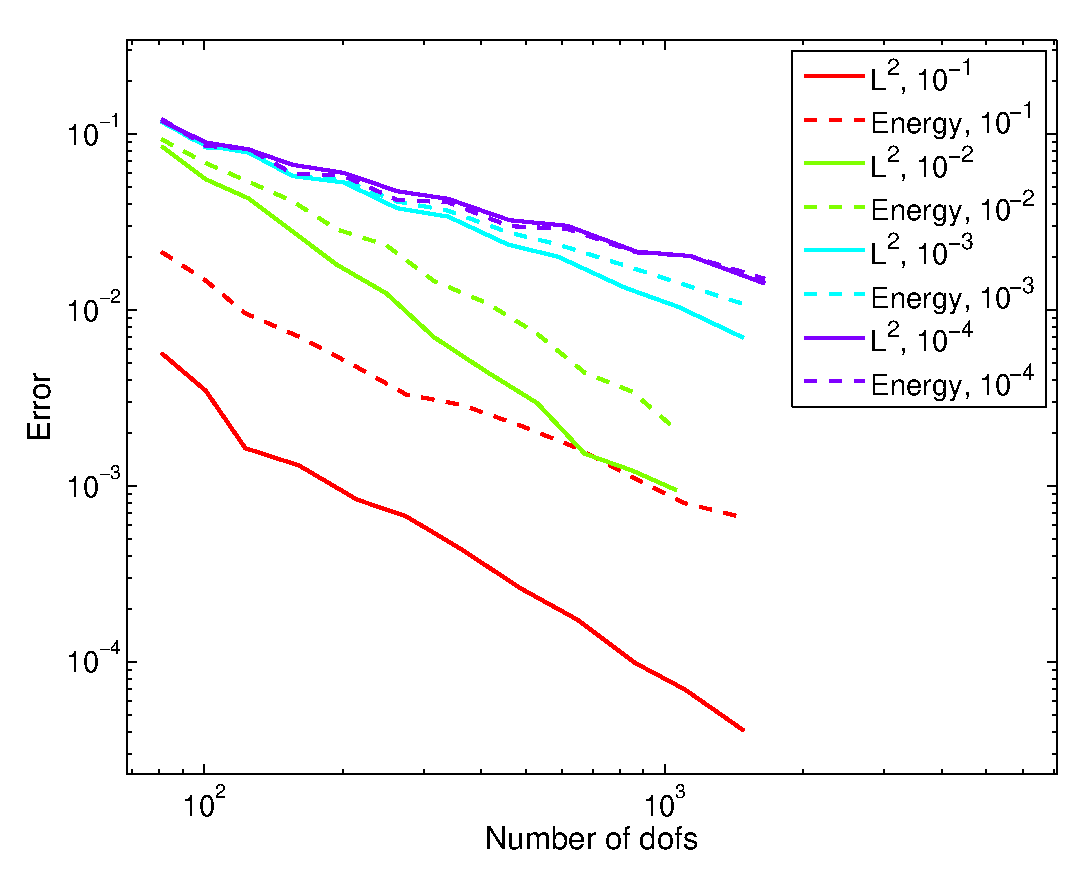
\includegraphics[scale=.6]{figs/epsRangeComparison.eps}
\caption{Comparison of $\L$ and energy error convergences under adaptive refinement for the Erikkson-Johnson problem for $\epsilon = 10^{-1}, 10^{-2}, 10^{-3}, 10^{-4}$ and $p=2$.}
\label{fig:erikksonEpsComparison}
\end{figure}

\subsection{Discontinuous forcing and advection skew to mesh}

\begin{figure}[!h]
\centering
\subfigure[$p=1$]{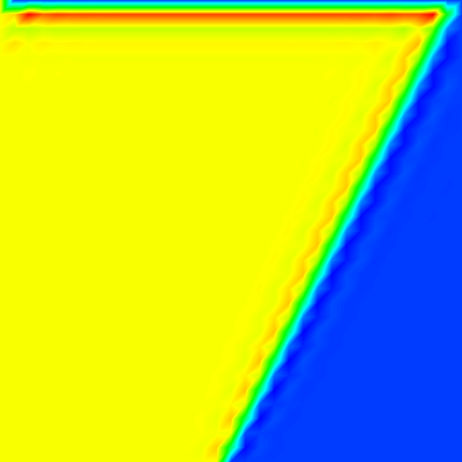
\includegraphics[width = .475\textwidth]{figs/skewToMeshP1Unif.png}}
\subfigure[$p=2$]{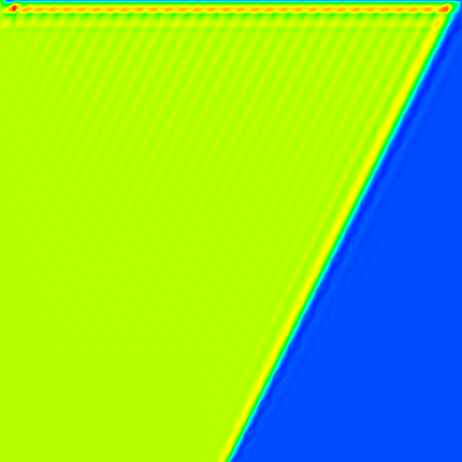
\includegraphics[width = .475\textwidth]{figs/skewToMeshP2Unif.png}}
\caption{Solution $u$ for advection skew to mesh with the upper-left hand corner discontinuity under both linear and quadratic uniform meshes.}
\label{fig:skewUnif}
\end{figure}
We examine first advection skew to the mesh, a common benchmark problem for convection-diffusion.  
\[
u = \begin{cases}
1 \text{ if } x = 0 \text{ or } y = 0 \text{ and } x< .5\\
0 \text{ otherwise},
\end{cases}
\]
Under such an example, a boundary layer develops at the outflow boundaries $x,y = 1$, and an internal layer develops due to the fact that the discontinuity in $f$ is parallel to the streamline.  We note that under the uniform meshes in Figure~\ref{fig:skewUnif} the method appears to deliver similar results to SUPG, and the discontinuity is convected across the domain in a minimially diffusive manner.  We avoid the use of adaptive meshes for this problem; since there exists a discontinuity in the outflow boundary conditions at the top left corner of the domain, adaptive mesh refinement schemes will tend to place a large number of refinements near this discontinuity, while not improving resolution of the salient features of the solutions (boundary and interior layers) or decreasing error.\footnote{For solutions with strong discontinuities, the placement of extraneous refinements is related to the fact that, for Sobolev-like residual norms, mesh refinement at discontinuities can actually increase residual error (this is also referred to as the Lavrentiev phenomenon; see \cite{gerritsmaEuler} for related discussion).  Thus, the use of adaptive mesh refinement for error reduction under such a problem is ineffective. }

%We avoid both the above ``fixes'' in order to more cleanly demonstrate the behavior of automatic adaptive mesh refinement; however, we note that under the uniform meshes in Figure~\ref{fig:skewUnif}, or under adaptive refinement schemes that avoids the corner singularity, the method appears to deliver similar results to SUPG.  
\begin{figure}[!h]
\centering
\subfigure{\includegraphics[width=.32\textwidth]{figs/DiscontinuousForcing.png}}
\subfigure{\includegraphics[width=.32\textwidth]{figs/DiscontinuousForcingMesh.png}}
\subfigure{\includegraphics[width=.32\textwidth]{figs/DiscontinuousForcingZoom.png}}
\caption{Model problem with $\epsilon = 10^{-3}$ and discontinuous forcing $f$.}
\label{fig:discForcing}
\end{figure}

We consider next a slight variant of a model problem introduced by Hughes and Sangalli in \cite{HughesVMS}.  The domain $\Omega$ is again taken to be the unit square, $\beta$ is taken to be $\beta = [.5,1]$, and $\epsilon = 10^{-3}$.  Homogeneous Dirichlet boundary conditions are taken over the entire boundary, and the problem is driven by a discontinuous forcing term $f(x,y)$, where
\[
f(x,y) = \begin{cases}
1 \text{ if } y > 2x \\
0 \text{ otherwise}.
\end{cases}
\]
Under such an example, a boundary layer develops at the outflow boundaries $x,y = 1$, and an internal layer develops due to the fact that the discontinuity in $f$ is parallel to the streamline.  Unlike the example of advection skew-to-mesh, the solution lies in $H^1$, implying that a good adaptive mesh refinement scheme should effectively resolve both interior and boundary layers.  
Figure~\ref{fig:discForcing} displays the solution and mesh resulting from 16 automatic mesh refinement iterations.  
%Figure~\ref{fig:discForcing2} displays a zoom of the solution and convergence history of the energy error.
%\begin{figure}[!h]
%\centering
%
%\subfigure{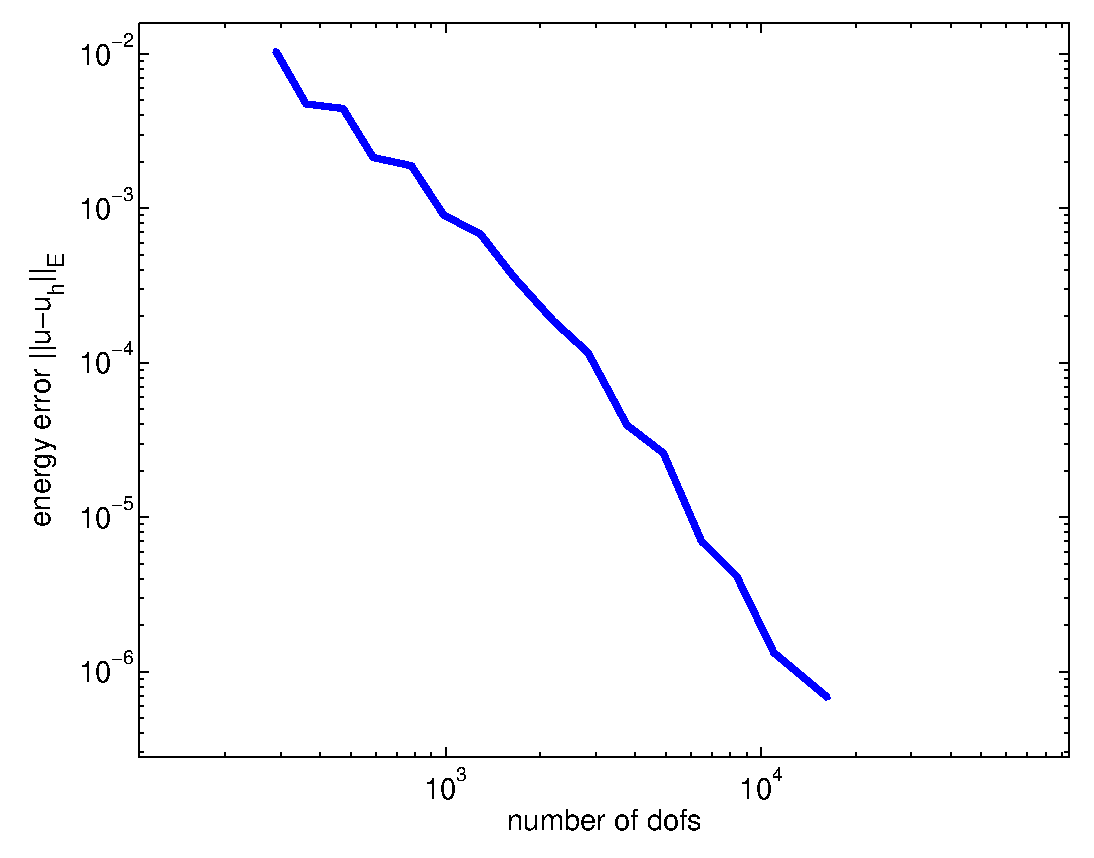
\includegraphics[scale=.45]{figs/rates/eps1e3DiscontinuousForcing.eps}}
%\caption{Zoom on the upper right-hand corner of the mesh for $f$ discontinuous.}%, along with convergence of energy error $\nor{u-u_h}_E$.}
%\label{fig:discForcing2}
%\end{figure}

%We adopt a modification of the standard problem parameters -- here, $\epsilon = 10^{-7}$, $\beta = [.5,1]$, and $f=0$.  Boundary conditions are set such that
%\[
%u = \begin{cases}
%1 \text{ if } y = 0, x< .5\\
%1-y \text{ if } x = 0\\
%0 \text{ otherwise}.
%\end{cases}
%\]
%Mathematically speaking, the considered problem is ill-posed for the standard Galerkin method in the continuous setting -- the boundary condition implies a discontinuity in $u$, such that the solution cannot lie in $H^1$.  The boundary condition is then convected in a manner that is skew to the mesh and forms a boundary layer on part of the outflow.
%
%\begin{figure}[!h]
%\centering
%\subfigure[Solution $u$]{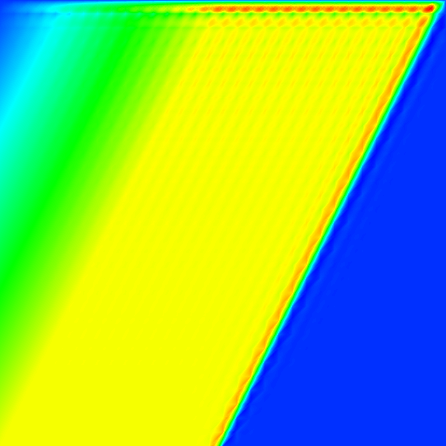
\includegraphics[scale=.3]{figs/skewToMesh.png}}
%\subfigure[$u$]{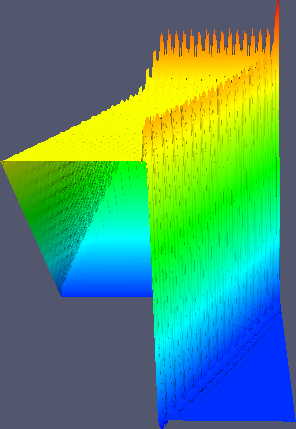
\includegraphics[scale=.313]{figs/skewToMesh3D.png}}
%\subfigure[Error representation $e$]{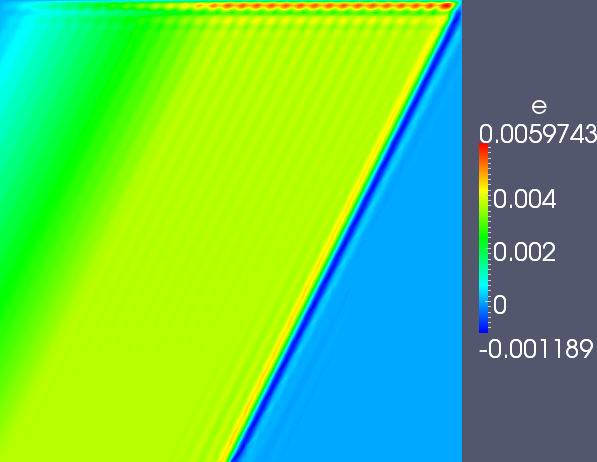
\includegraphics[scale=.29]{figs/skewToMeshE.png}}
%\caption{Advection skew to mesh on a uniform quadratic $32\times 32$ grid of triangles.  The fine scale error representation function $e$ is also shown; note that the multiscale contribution of $e$ is dependent on the form of $\LRp{e,v}_V$, which involves streamline derivatives.}
%\end{figure}
%
%\begin{figure}[!h]
%\centering
%\subfigure{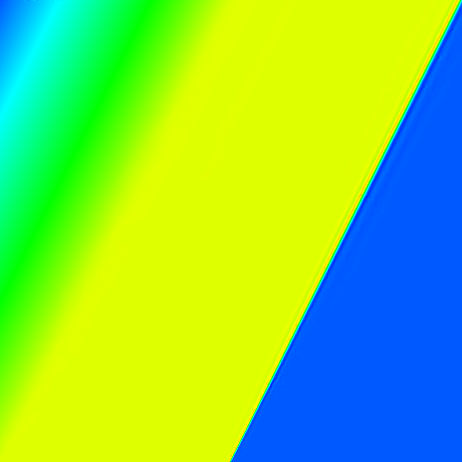
\includegraphics[scale=.43]{figs/skewToMeshAdapt.png}}
%\subfigure{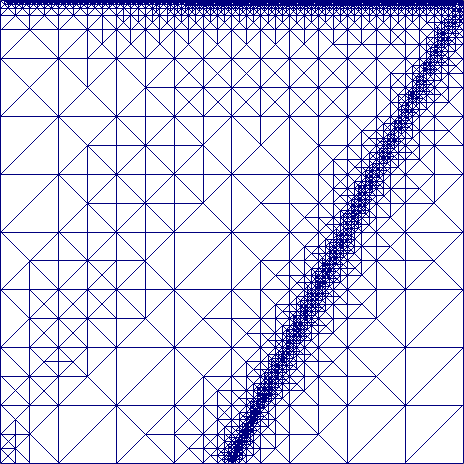
\includegraphics[scale=.43]{figs/skewToMeshAdaptMesh.png}}
%\caption{Advection skew to mesh after iterations 18 of adaptive mesh refinement.}
%\end{figure}
%
%%\begin{figure}[!h]
%%\centering
%%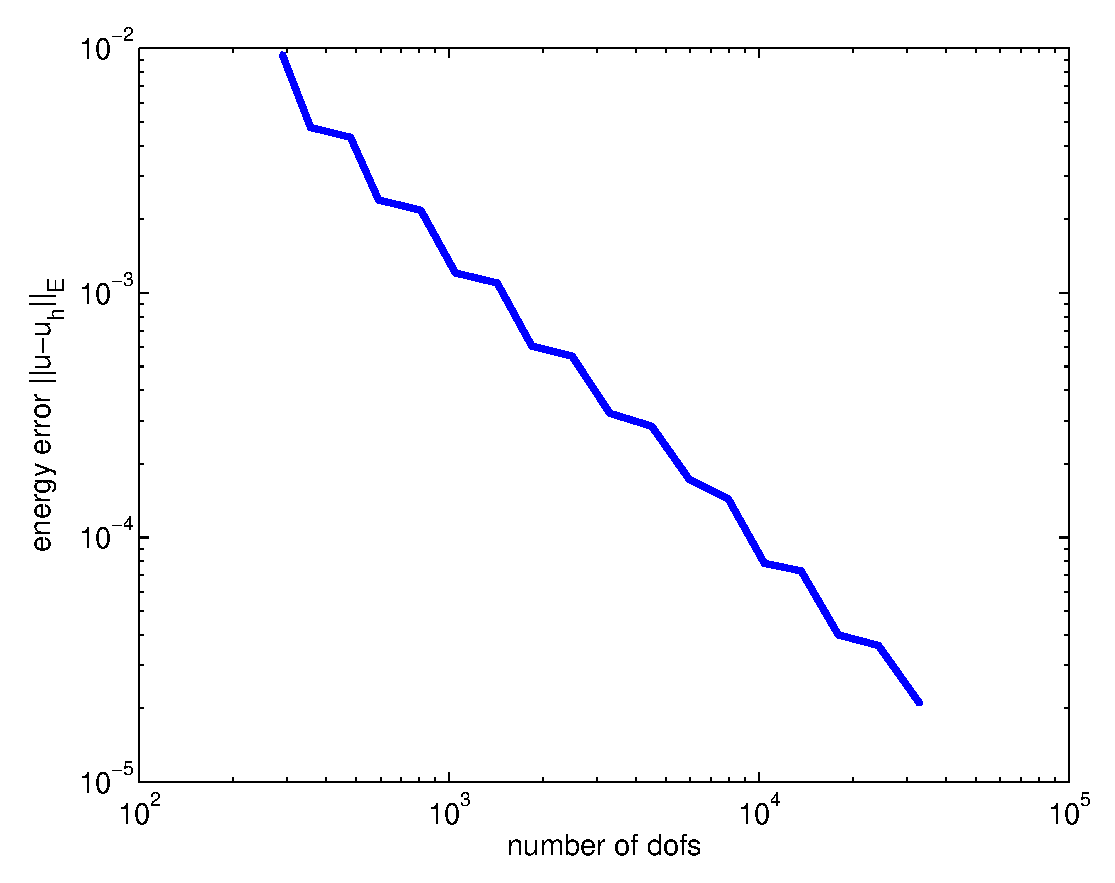
\includegraphics[scale=.45]{figs/rates/eps5e7SkewToMesh.eps}
%%\caption{Energy error for advection skew to mesh over 18 iterations of adaptive mesh refinement.}
%%\end{figure}

%We note that the standard boundary condition for advection skew to the mesh is 

%\subsection{A 3D model problem}
%
%We conclude by applying the method to a simple model problem in 3 space dimensions.  We solve on the unit cube $\Omega = [0,1]^3$ with $\beta = [1,1,1]$, $f=1$ and $u=0$ on $\partial \Omega$.  A boundary layer develops on the outflow boundaries $x,y,z = 1$.  Figure~\ref{fig:3D5e2} displays slices of the domain along the streamline direction to illustrate the formation of such a boundary layer.  
%
%\begin{figure}[!h]
%\centering
%\subfigure{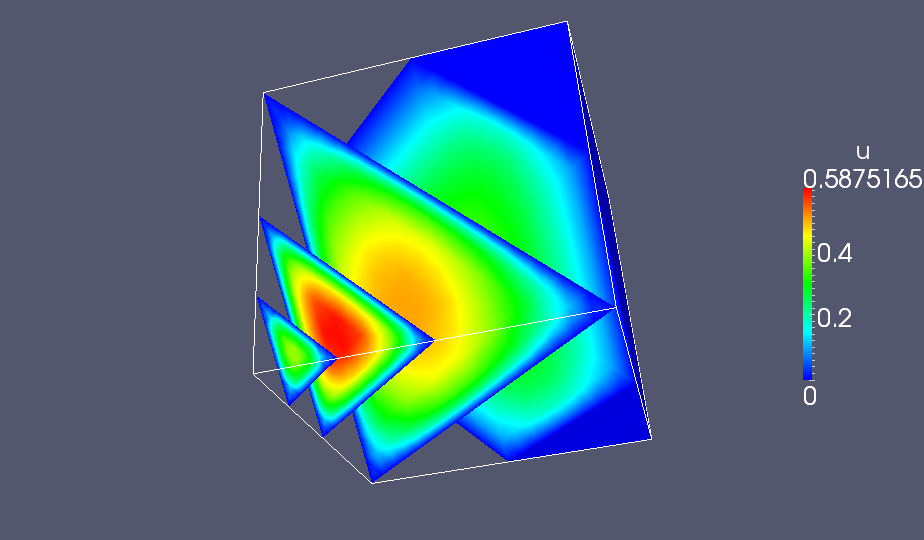
\includegraphics[scale=.44]{figs/3DSlices5e2.png}}
%\caption{3D Model problem with $\epsilon = 5e-2$.}
%\label{fig:3D5e2}
%\end{figure}
%
%We examined the behavior of the method with respect to a small $\epsilon$, in this case $\epsilon = 10^{-6}$.  8 adaptive refinements were done beginning with a uniform linear mesh of 8 elements per side; Figure~\ref{fig:3D1e6} shows the resulting solution and mesh along a cut orthogonal to the streamline direction.  All experiments indicate that the method appears to behave qualitatively the same as in 2 dimensions, modulo increased computational cost.
%
%\begin{figure}[!h]
%\centering
%%\subfigure{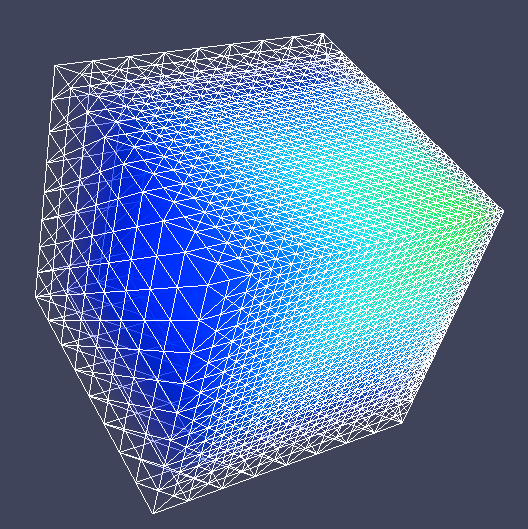
\includegraphics[scale=.25]{figs/3DMesh.png}}
%\subfigure{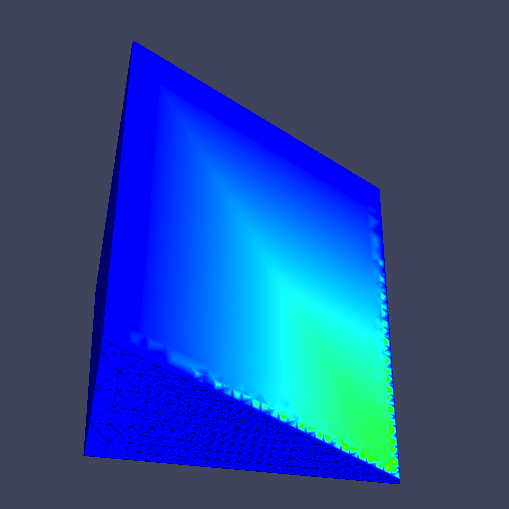
\includegraphics[scale=.4]{figs/3DSlice.png}}
%\subfigure{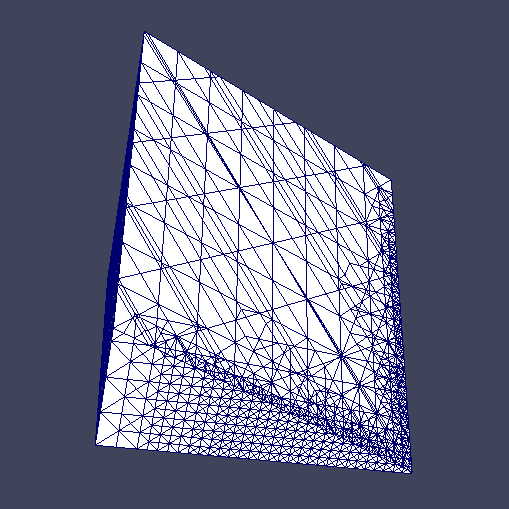
\includegraphics[scale=.4]{figs/3DMeshSlice.png}}
%\caption{3D Model problem with $\epsilon = 10^{-6}$ after 8 refinements.  The cube is sliced along a plane with normal direction orthogonal to the streamline in order to illustrate the clustering of refinements in the interior of the domain.}
%\label{fig:3D1e6}
%\end{figure}
%
%%\textcolor{red}{Does Hughes have a reference for the weakening of divergence in higher dimensions?}.  

\subsection{Weak boundary conditions and comparison to other methods}

We close by introducing a method for the weak imposition of boundary conditions.  For stability reasons, we modified the variational formulation with an additional boundary term on the inflow boundary.  If we take instead 
\begin{align*}
\delta u, u &\in H^{\frac{3}{2}+\delta}(\Omega) \cap H^1_{\rm in} \\
e,v &\in H^{\frac{3}{2}+\delta}(\Omega) \cap H^1_{\rm out}
\end{align*}
where $H^1_{\rm in} \coloneqq \LRc{v\in H^1(\Omega) s.\ t.\ \left.v\right|_{\Gamma_{\rm in}} = 0}$, we can weakly impose the outflow boundary by modifying the variational formulation used in the saddle point system in Section~\ref{sec:saddlePoint}.  The resulting variational formulation is 
\[
b(u,v) = (\Grad u, \beta v + \epsilon \Grad v)_{\L} - \epsilon\int_{\Gamma_{\rm in}} \pd{u}{n}v - \epsilon\int_{\Gamma_{\rm out}} \pd{v}{n} u = (f,v)_{\L}, \quad \forall v \in V_h.
\]
Figure~\ref{fig:weakBCs} demonstrates the release of the outflow boundary condition as ${\epsilon}$ vanishes relative to the mesh size: for a sufficiently resolved mesh with $\epsilon \approx h$, the boundary condition activates, but releases as the ratio $\epsilon/h \rightarrow 0$.  Taking $\epsilon = 0$ convergences to a stable method for the pure convection equation.  
%The nonsymmetric Nitsche was shown to be stable without a penalty term in \cite{penaltyFreeNitsche}; however, 
\begin{figure}
\centering
\subfigure{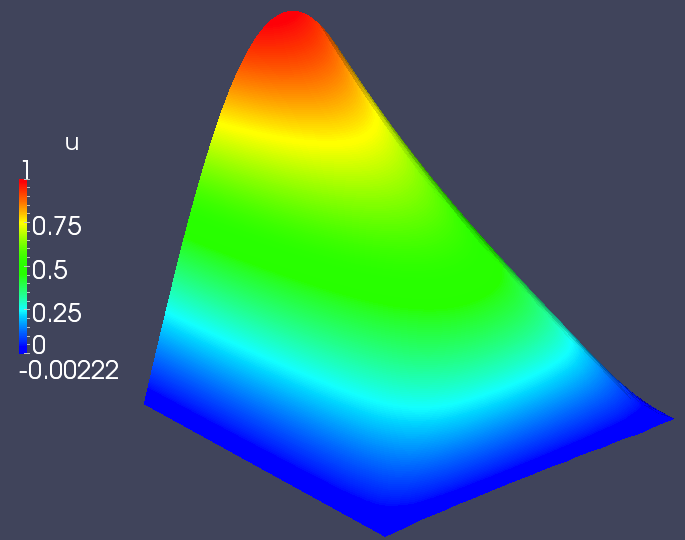
\includegraphics[width = .24\textwidth]{figs/weakBCs/eps1e1.png}}
\subfigure{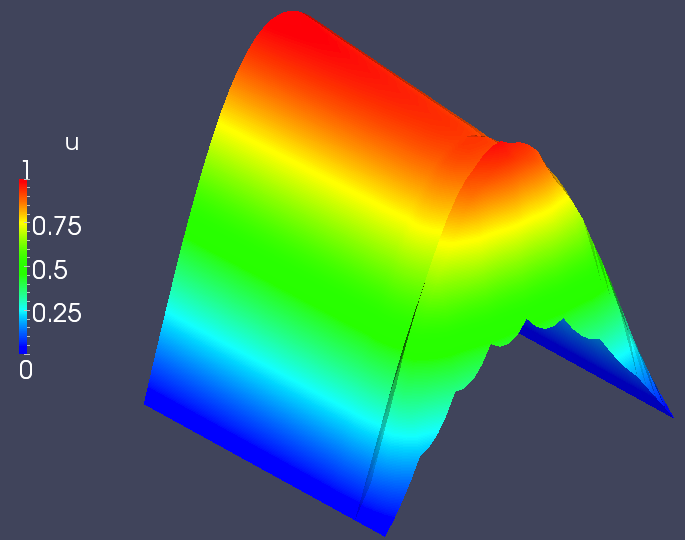
\includegraphics[width = .24\textwidth]{figs/weakBCs/eps1e2.png}}
\subfigure{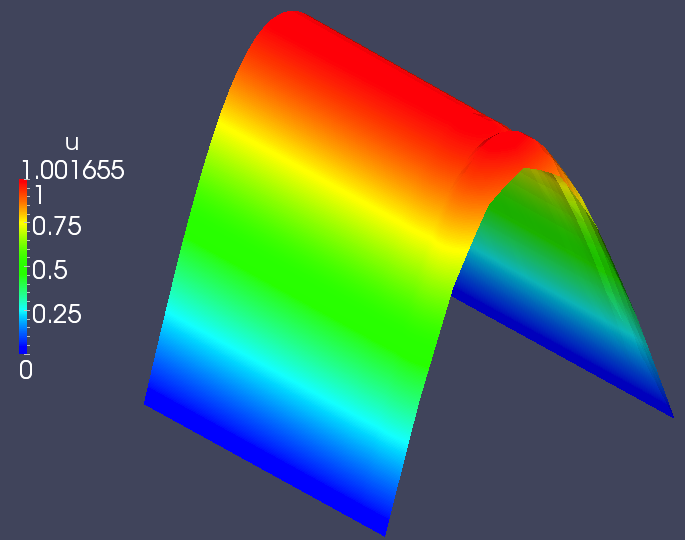
\includegraphics[width = .24\textwidth]{figs/weakBCs/eps1e3.png}}
\subfigure{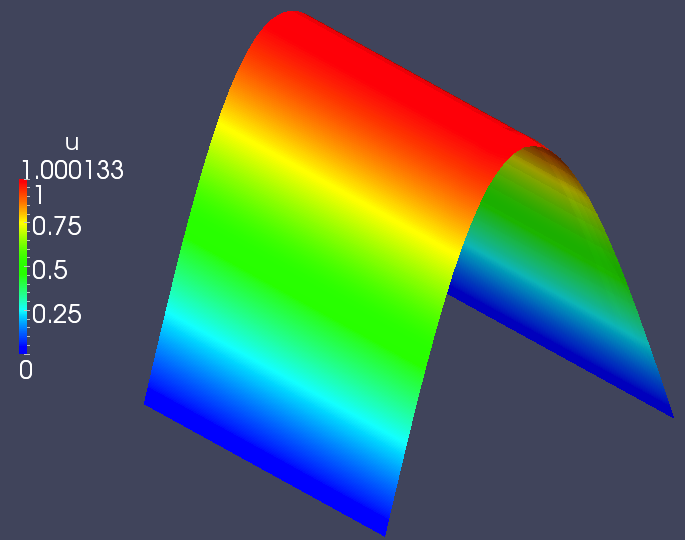
\includegraphics[width = .24\textwidth]{figs/weakBCs/eps1e4.png}}
\caption{Weak boundary imposition for $\epsilon = 10^{-1}, 10^{-2}, 10^{-3}, 10^{-4}$.}
\label{fig:weakBCs}
\end{figure}	

Figure~\ref{fig:supg_comparison} compares the convergence of $L^2$ error with SUPG\footnote{The stabilization parameter is taken to be $\tau = \frac{h}{\LRb{\beta}(p+1)}$ in this comparison.} to this method under both the strong and weak imposition of boundary conditions.  While the rate of convergence does not change, the imposition of a weak outflow boundary condition greatly decreases the $L^2$ error.  We note that the asymptotic rate of convergence is less than the optimal rate for $p=4$; however, increasing to $\triangle p = 2$ recovers the optimal rate.  
\begin{figure}
\centering
\subfigure[$\epsilon = 1.0$]{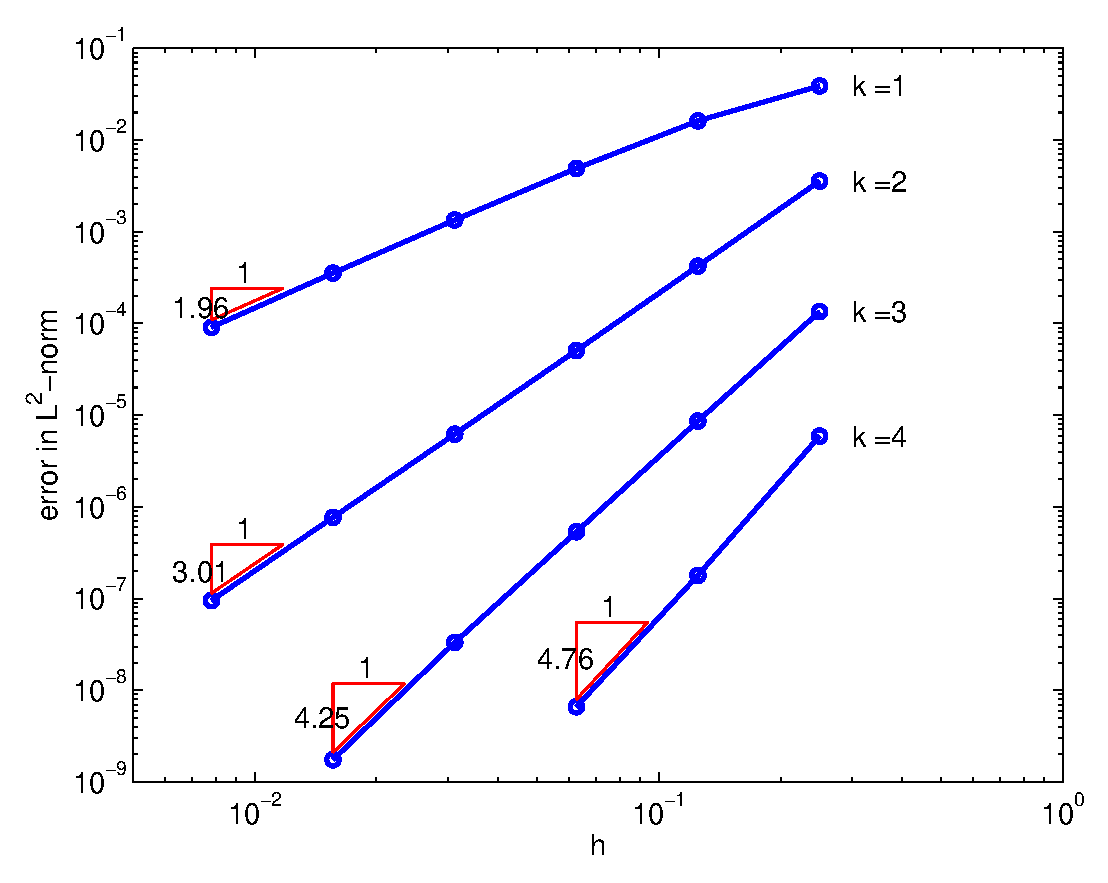
\includegraphics[width = .475\textwidth]{figs/rates/eps1e0Rates_weakBC.eps}}
\subfigure[$\epsilon = 10^{-4}$, $p=1$]{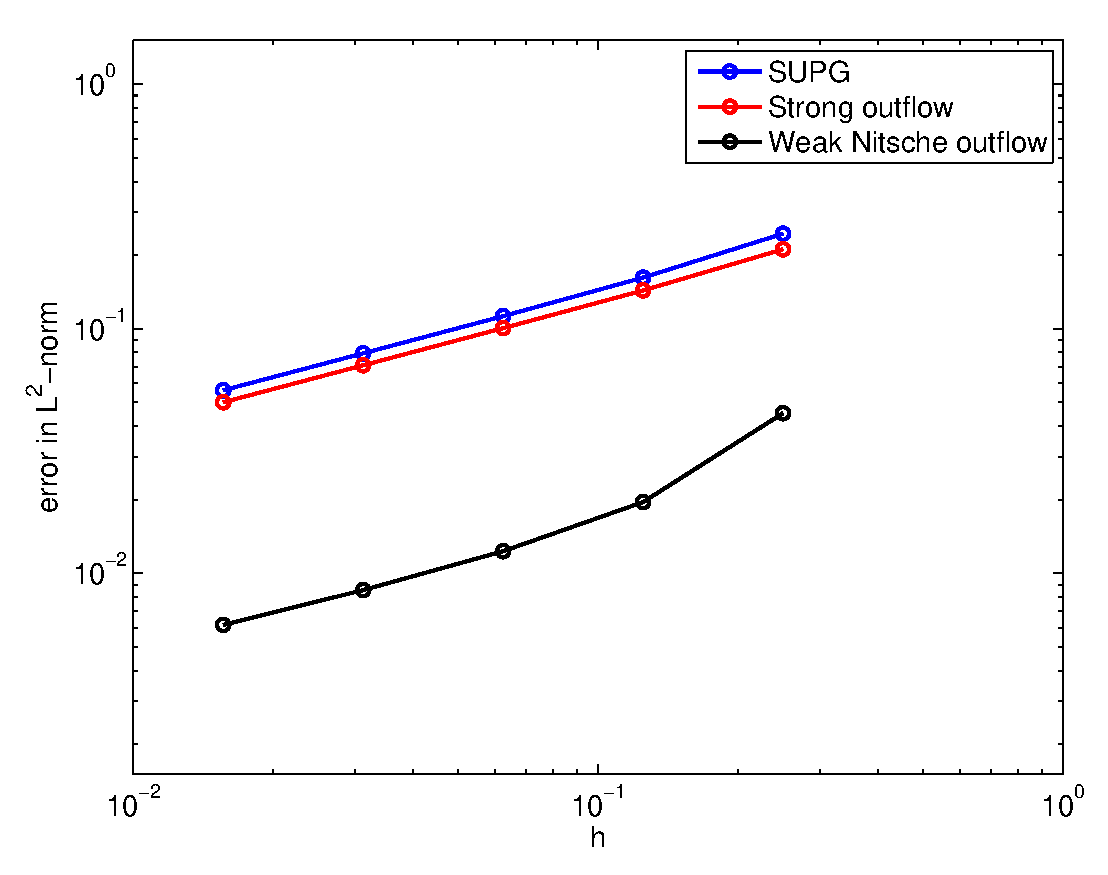
\includegraphics[width = .475\textwidth]{figs/rates/supg_bc_comparison.eps}}
\caption{Convergence rates for the diffusive regime, and comparison between methods (for $p=1$) under uniform refinement for convective regime.}
\label{fig:supg_comparison}
\end{figure}	

\section{Conclusions and future direction}

We have presented a higher order adaptive $H^1$-conforming method for convection-diffusion problems for very small $\epsilon$, and have made connections to both the DPG method as well as the method of Cohen, Dahmen and Welper.  The method has also been shown to be derivable in the Variational Multiscale framework as well, and is distinguished from traditional VMS methods in its definition of the fine-scale space and problem.  Unlike standard stabilized methods, there are no stabilization parameters to specify.  %However, unlike the DPG methods of both Demkowicz and Gopalakrishnan, as well as the method of Broersen and Stevenson, this method is easily implementable within current finite element codes in arbitrary spatial dimensions.

We note that, while the method displays similarities to SUPG, we do not observe nodal exactness in 1D.  The two methods differ in that we do not work directly with coarse scales defined by the $H^1$ inner product; unless we can induce an energy inner product such that $\LRp{u_h,u'}_E = \LRp{u_h,u'}_{H^1_0}$, then we should not expect nodal exactness in 1D.  However, in higher space dimensions, the behavior of the method is qualitatively very similar to SUPG.  

%We hope to explore in future research both additional improvements on the method and the application of this method to other problem frameworks and settings, a few of which are described in the following sections.  

%\subsection{$hp$-refinement}
%
Since this method is derived from the same variational principles as DPG, it should likewise be automatically inf-sup stable for arbitrary $hp$ meshes as well.  $hp$-refinement is of interest due to the fact that, under proper choices between $h$ and $p$ refinement, exponential convergence rates are possible, and have been observed for several model problems \cite{demkowicz2006computing}.  %Intelligent $hp$-adaptive strategies could also offer more mathematically motivated alternatives to CFD approaches such as flux limiters, which effectively limit the order of approximation in areas of singularities and high gradients.  
%
%Additionally, the method automatically extends to incorporate anisotropic elements and $r$-refinement as well, similar to ALE methods.  The combination of these two methods has been shown to produce very fine-resolution results at a competitive computational cost for flow problems with very small viscosity \cite{AlmeidaAnisotropy}.  

\subsection{Computational feasibility}

The main obstacle to making this method computationally competitive is the doubling of the number of fully coupled degrees of freedom in solving the problem in saddle point system formulation.  While a larger number of degrees of freedom is often cited as a detriment, it is often accompanied by an advantageous underlying structure -- for example, discontinuous Galerkin methods are also often criticized for their ``explosion of degrees of freedom'' compared to continuous Galerkin methods \cite{cottrell2007isogeometric}, but their local nature aids significantly in parallelization, adaptivity, and explicit time integration, as opposed to methods based on continuous discretizations.  

The cost of explicitly discretizing the fine scale error representation $e\in V_h$ roughly amounts to the cost of discretizing an additional coupled PDE under a higher resolution.   The idea of solving an additional PDE for the purposes of stabilization is not unheard of \cite{Barter}; however, the additional discretization cost must be minimized, or at least offset by additional positive properties of the resulting system.  We propose several preliminary ideas for doing so: 
\begin{itemize}
%\item Recall in Section~\ref{sec:saddlePoint} that the saddle point system is reducible to 
%\[
%\bs{B}^T \bs{A}^{-1}\bs{B} \bs{u} = \bs{B}^T \bs{A}^{-1}\bs{f}.
%\]
%where $f$ and $B$ are the load and overdetermined stiffness matrix under $V_h$, and $A$ is the Gram matrix/discrete Riesz map associated with the inner product $\LRp{v,\delta v}_V$.  One approach is to explore possibilities for rapid inversion of $A$.  For example, it is possible to choose $V_h$ to simply be the space of piecewise linears enriched with bubbles -- higher order degrees of freedom could be condensed out, resulting in a system for $e$ with the same number of unknowns as $u$.  The resulting matrix-vector products required to form the Schur complement could be parallelized as well.  

%One additional possibility would be the exploration of iterative methods for the Schur complement -- the matrix is positive definite, and assembling a matrix-vector product could be done efficiently under a good preconditioner for the symmetric positive-definite matrix $\bs{A}^{-1}$.  Preliminary results demonstrate effective speedup for uniform meshes of piecewise linears in 2D using standard preconditioners (ILU, block Jacobi, AMG), and suggest that a discretization of $V_h$ using a $h$-refined fine mesh could be possible; however, more work would be required to develop preconditioners for high order adaptive meshes.  
%\item Another possibility would be to solve the saddle point problem using an Uzawa method \cite{uzawa}, which would decouple the saddle point system into two problems, each involving only degrees of freedom for $e$ or for $u$.  The solution of these two problems feeds an iterative procedure which can converge to the solution of the saddle point problem.  Again, effective use of an Uzawa algorithm would require a good preconditioner for $\bs{A}$ under high-order refined meshes.
\item Dahmen, Huang, Schwab, and Welper utilize an iterative Uzawa method for the pure convection equation, which allows for the separate solution of two symmetric, coercive problems for $u$ and $e$ \cite{dahmenConvection}.  Dahmen et al.\ showed that the trial norm induced by their choice of test norm is precisely the $L^2$ norm, and utilized this in their Uzawa iteration.  However, to use an Uzawa iteration for the convection-diffusion equation for $\epsilon > 0$ would require an explicit expression of the induced trial norm, which has not yet been derived in closed form.  
\item We hope to explore alternative discretizations for both $U_h$ and $V_h$ in order to minimize degrees of freedom or solution for in the overall system.  A few examples of nonstandard discretizations include higher order continuity basis functions (splines and NURBS \cite{NURBSorig}), and discontinuous functions (DG).  Preliminary experiments have yielded promising results in 1D under the combination of higher-continuity and $C_0$ bases for $U_h$ and $V_h$, respectively.  We hope to further explore intelligent mixing of discretizations for trial and test spaces in future experiments.  
\item The DPG method achieves computational efficiency by block-diagonalizing $\bs{A}$ using discontinuous test functions and trace/flux degrees of freedom on element boundaries.  The same method could be applied to the $H^1$ setting for convection-diffusion problems at the cost of introducing inter-element fluxes representing the trace on the boundary of an element resulting from integration by parts of the viscous term, similarly to the primal DPG method \cite{primalDPG}.  An alternative along the same lines would be to consider block diagonalization of $\bs{A}$ under a patch-based decomposition, such as FETI or one of its variants \cite{FETI1,FETI2}.  Both of these methods would allow for more efficient inversion of $\bs{A}$ in the computation of the symmetric positive-definite Schur complement $\bs{B}^T \bs{A}^{-1} \bs{B}$ at the cost of introducing additional hybrid unknowns on element faces.  This method is akin to approximating the error representation $e$ using a nonconforming primal hybrid finite element method \cite{raviart1977primal}.  
\end{itemize}

\section{Acknowledgements}

The authors would like to acknowledge the help of Truman Ellis and Dr.\ Leszek Demkowicz for fruitful discussions and perspective.  Jesse Chan was supported by the Department of Energy [National Nuclear Security Administration] under Award Number [DE- FC52-08NA28615].  John A.\ Evans was partially supported by the ICES Postdoctoral Fellowship at the Institute for Computational Engineering and Sciences, and by a grant from the Office of Naval Research [N00014-08-1-0992].   Weifeng Qiu was supported by the City University of Hong Kong under start-up grant No. 7200324.

\bibliographystyle{unsrt}
\bibliography{paper}


\end{document}
